\pagestyle{plain}

\subsection{Generalities}
	\label{ss:DefAn} In this section, we recall the precise description of $\rep(Q)$ for $Q$ a type $A$ quiver.
	
\begin{definition} \label{def:Antype}
    Let $n \in \mathbb{N}^*$. A quiver $Q$ is of $A_n$ type if the underlying graph of $Q$ is of the following shape.
    \begin{center}
		\begin{tikzpicture}[-,line width=0.5mm,>= angle 60,color=black,scale=0.8]
			\node (1) at (0,0){$1$};
			\node (2) at (2,0){$2$};
			\node (3) at (4,0){$\cdots$};
			\node (4) at (6,0){$n$};
			\draw (1) -- (2) -- (3) -- (4);
		\end{tikzpicture}
	\end{center}
\end{definition}
 
Let $n \in \mathbb{N}^*$. The \new{intervals} of $\{1, \ldots, n\}$ are the sets $\llrr{i,j} := \{i, i+1, \ldots,j \}$ given by all $1 \leqslant i \leqslant j \leqslant n$. If $i=j$, we write $\llrr{i,i} = \llrr{i}$. Denote by $\mathcal{I}_n$ the set of intervals in $\{1, \ldots n\}$. For $K = \llrr{i,j} \in \mathcal{I}_n$, set $b(K) = i$ and $e(K) = j$. Call \new{interval set} any subset of $\mathcal{I}_n$.
	\begin{definition}\label{def:intervalbotandtop}  Let $Q$ be an $A_n$ type quiver. Consider $K,L \in \mathcal{I}_n$ such that $K \subseteq L$. We say that:
		\begin{enumerate}[label = $\bullet$]
			\item $K$ is \new{above} $L$ (\new{relative to} $Q$) if the two following assertions are satisfied:\begin{enumerate}[label = $\bullet$]
				\item $b(K) = b(L)$ or we have the arrow $b(K)-1 \longleftarrow b(K)$ in $Q$;
				\item $e(K) = e(L)$ or we have the arrow $e(K) \longrightarrow e(K)+1$ in $Q$.
			\end{enumerate}
			\item $K$ is \new{below} $L$ (\new{relative to} $Q$) if the two following assertions are satisfied:\begin{enumerate}[label = $\bullet$]
				\item $b(K) = b(L)$ or we have the arrow $b(K)-1 \longrightarrow b(K)$ in $Q$;
				\item $e(K) =e(L)$ or we have the arrow $e(K) \longleftarrow e(K)+1$ in $Q$.
			\end{enumerate}
		\end{enumerate}
	\end{definition}
	\begin{ex} Consider the following quiver.
		\begin{center}
			\begin{tikzpicture}[->,line width=0.5mm,>= angle 60,color=black,scale=0.8]
				\node (Q) at (-1,0){$Q =$};
				\node (1) at (0,0){$1$};
				\node (2) at (2,0){$2$};
				\node (3) at (4,0){$3$};
				\draw (1) -- (2);
				\draw (2) -- (3);
			\end{tikzpicture}
		\end{center}
		Then $\llrr{2}$ is above $\llrr{2,3}$ and below $\llrr{1,2}$.
	\end{ex}
	Note that any interval is above and below itself, relative to all $A_n$ type quivers.
	Let $Q$ be a quiver of $A_n$ type. To any interval $K \in  \mathcal{I}_n$, we consider $X_K$ the representation of $Q$ defined as it follows:
	\begin{enumerate}[label = $\bullet$]
		\item $(X_K)_q = \mathbb{K}$ if $q \in K$, $(X_K)_q = 0$ otherwise;
		\item $(X_K)_{\alpha} = \Id_\mathbb{K}$ if $\alpha$ is such that $\{s(\alpha), t(\alpha)\} \subseteq K$, $(X_K)_{\alpha} = 0$ otherwise;
	\end{enumerate}
	Note that $X_K$ is an indecomposable representation of $Q$ for all $K \in \mathcal{I}_n$.
	\begin{theorem}\label{thm:indecandmorphtypeA} Let $Q$ be an $A_n$ type quiver. \begin{enumerate}[label = $(\alph*)$]
			\item \label{indectypeA} The isomorphism classes of indecomposable representations of $Q$ are in bijection with $\mathcal{I}_n$; more precisely, they are described by indecomposable representations $X_K$ for $K \in \mathcal{I}_n$;
			\item \label{morphtypeA} The homomorphism space between two indecomposable representations of $Q$ is of dimension at most one; more precisely, $\Hom(X_K, X_L)$ is nonzero if and only if  there exists an interval $J$ such that $J$ is above $K$ and below $L$ relative to $Q$; if such an interval exists, it is unique and 
			$\Hom(X_K,X_L)$ consists of scalar multiples of the morphism $\phi = (\phi_q)_{q \in Q_0}$ such that $\phi_q = \Id_\mathbb{K}$ if $q \in J$ and $\phi_q = 0$ otherwise. 
		\end{enumerate}
	\end{theorem}
	In the light of the previous result : \begin{enumerate}[label = $\bullet$]
		\item for all interval sets $\mathscr{J} \subseteq \mathcal{I}_n$ and all quivers $Q$ of $A_n$ type, write $\Cat_Q(\mathscr{J})$ the subcategory of $\rep(Q)$ additively generated by $X_K$ for $K \in \mathscr{J}$;
		\item for all quivers $Q$ of $A_n$ type and for all nonzero subcategories $\mathscr{C}$ of $\rep(Q)$, let $\Int(\mathscr{C})$ be the interval set of $\mathcal{I}_n$ consisting of intervals $K$ such that $X_K \in \mathscr{C}$.
	\end{enumerate}
	Under \cref{conv:addsubcat}, the subcategories we are considering are additively generated by $X_K$ for $K \in \mathscr{J}$ for some  $\mathscr{J} \subset \mathcal{I}_n$.
	
	Hence, for any $A_n$ type quiver $Q$, for all $\mathscr{J} \subseteq \mathcal{I}_n$ and for all subcategories $\mathscr{C} \subseteq \rep(Q)$, we have $\mathscr{J} = \Int(\Cat_Q(\mathscr{J})) \text{ and } \mathscr{C} = \Cat_Q(\Int(\mathscr{C})).$

    Now we recall the description of all the short exact sequences between indecomposable representations.

    \begin{theorem} \label{thm:exttypeA} Let $Q$ be an $A_n$ type quiver. Let $D,F \in \ind(Q)$ and consider a non-split exact sequence \[\begin{tikzcd}
	0 & D & E & F &  0.
	\arrow[from=1-1, to=1-2]
	\arrow[tail, from=1-2, to=1-3]
	\arrow[two heads,from=1-3, to=1-4]
	\arrow[from=1-4, to=1-5]
\end{tikzcd} \]
      Then exactly one of the following assertions holds:
      \begin{enumerate}[label=$(\alph*)$,itemsep=1mm]
          \item We have $E \in \ind(Q)$, and if we consider $K,L \in \mathcal{I}_n$ such that $D \cong X_K$ and $F \cong X_L$, then $K \cup L \in \mathcal{I}_n$, $K \cap L = \varnothing$ and $E \cong X_{K \cup L}$; or,
          \item We have $E \cong E_1 \oplus E_2$ with $E_1,E_2 \in \ind(Q)$, and there exist $K,L \in \mathcal{I}_n$ with $K \cap L \neq \varnothing$ such that both assertions hold:
          \begin{enumerate}[label=$\bullet$,itemsep=1mm]
          \item $K,L,K \cap L$ and $K \cup L$ are four different intervals in $\mathcal{I}_n$; and,
          \item either $\{D,F\} = \{X_K, X_L\}$ and $\{E_1,E_2\} = \{X_{K\cap L}, X_{K \cup L} \}$, or \\
          $\{D,F\} = \{X_{K \cap L}, X_{K \cup L}\}$ and $\{E_1,E_2\} = \{X_{K}, X_{L} \}$.
          \end{enumerate}
          In this case, we call it a \new{diamond exact sequence.} 
      \end{enumerate}
    
    \end{theorem}
    
We recall the following crucial notion.

\begin{definition} \label{def:directing}
    Let $\mathscr{A}$ be an abelian category. We say that $\mathscr{A}$ is \new{directing} if both of the following assertions hold:
    \begin{enumerate}[label=$\bullet$, itemsep=1mm]
        \item for any sequence of nonzero objects $(V_i)_{i \in \mathbb{N}}$ of such that, for all $i \in \mathbb{N}$, there exists a nonzero morphism $f_i : V_{i+1} \longrightarrow V_{i}$, there exists $m \in \mathbb{N}$ such that for all $i \geqslant m$, the morphism $f_i$ is an isomorphism; and,
        \item for any sequence of nonzero objects $(V_i)_{i \in \mathbb{N}}$ of such that, for all $i \in \mathbb{N}$, there exists a nonzero morphism $g_i : V_{i} \longrightarrow V_{i+1}$, there exists $m \in \mathbb{N}$ such that for all $i \geqslant m$, the morphism $g_i$ is an isomorphism; and,
    \end{enumerate}
\end{definition}

\cref{def:directing} is a restatement of the usual definition. See \cite{ASS06} for more details.

\begin{theorem} \label{thm:Andirecting}
    Let $Q$ be an $A_n$ type quiver for some $n \in \mathbb{N}^*$. Then $\rep(Q)$ is directing.
\end{theorem}

Finally, we will focus on a special exact structure on $\rep(Q)$.

\begin{definition} \label{def:Ediamond}$ $
Let \( Q \) be an $A_n$ type quiver for some $n \in \mathbb{N}^*$. The \new{diamond exact structure} $\mathcal{E}_{\diamond}$ on $\rep(Q)$ is defined as the collection of all classes of short exact sequences that can be expressed as direct sums of split short exact sequences and diamond exact sequences.
\end{definition}

\begin{prop}[\cite{BHRS24}]
 \label{prop:EdiamondExactStructureTypeA}
     Let $n \in \mathbb{N}^*$, and $Q$ be an $A_n$ type quiver. The collection $\mathcal{E}_{\diamond}$ is an exact structure on $\mathscr{A} = \rep(Q)$.
 \end{prop}


\subsection{Diamond exact structure and tilting representations}
\label{ss:Diamond}
In the following, we fix the following setting.

\begin{conv}\label{conv:typeA}
    We fix $Q$ an $A_n$ type quiver, for some $n \in \mathbb{N}^*$. We endow $\rep(Q)$ with an exact structure $\mathcal{E}$.
\end{conv}

Denote by $\Tilt(Q)$ the collection $\Tilt(\rep(Q))$. In this section, we establish a strong link between $\mathcal{E}_\diamond$-adapted extension-closed subcategories and the tilting representations. First, let us show the following result.

\begin{theorem}
\label{thm:maximal}
 Let $T \in \Tilt(Q)$. Then $\GS_{\mathcal{E_\diamond}}(T)$ is a maximal (for inclusion) $\mathcal{E}_\diamond$-adapted subcategory closed under extensions.
\end{theorem}

\begin{proof}
Assume by absurdity that such a subcategory $\mathscr{C} \supsetneq \GS_{\mathcal{E}_\diamond}(T)$ exists. By \cref{conv:addsubcat}, there exists $V \in \ind(Q)$ such that $V \in \mathscr{C}$ and $V \notin \GS_{\mathcal{E}_\diamond}(T)$.

As $\mathscr{C}$ is $\mathcal{E}_\diamond$-adpated, we have that $\Ext^1(\mathscr{C},V)$ and $\Ext^1(V,\mathscr{C})$ are contained in $\mathcal{E}_\diamond$. As $T$ is tilting, then there exist an indecomposable direct summand $T_0$ of $T$ such that there is a non-split short exact sequence \[\begin{tikzcd}
	\xi_0: & 0 & T_0 & E_0 & V &  0 & \in \mathcal{E}_\diamond,
	\arrow[from=1-2, to=1-3]
	\arrow[tail, from=1-3, to=1-4]
	\arrow[two heads,from=1-4, to=1-5]
	\arrow[from=1-5, to=1-6]
\end{tikzcd}\]  or \[\begin{tikzcd}
	\varsigma_0: & 0 & V & E_0 & T_0 &  0 & \in \mathcal{E}_\diamond.
	\arrow[from=1-2, to=1-3]
	\arrow[tail, from=1-3, to=1-4]
	\arrow[two heads,from=1-4, to=1-5]
	\arrow[from=1-5, to=1-6]
\end{tikzcd}\]

Assume that we have $\xi_0 \in \mathcal{E}_\diamond$. By construction, we have that $\Gen_{\mathcal{E}_\diamond}(\GS_{\mathcal{E}_\diamond}(T)) \subseteq \GS_{\mathcal{E}_\diamond}(T)$. Therefore, there must be one of the indecomposable summands of $E_0$, let us call it $V_1$, that is not in $\GS_{\mathcal{E}_\diamond}(T)$. On the other hand, $\mathscr{C}$ is extension closed, and so $V_1 \in \mathscr{C}$. By the same arguments than those applied to $V$ previously, there exists an indecomposable direct summand $T_1$ of $T$ such that there is a non-split short exact sequence \[\begin{tikzcd}
	\xi_1: & 0 & T_1 & E_1 & V_1 &  0 & \in \mathcal{E}_\diamond,
	\arrow[from=1-2, to=1-3]
	\arrow[tail, from=1-3, to=1-4]
	\arrow[two heads,from=1-4, to=1-5]
	\arrow[from=1-5, to=1-6]
\end{tikzcd}\]  or \[\begin{tikzcd}
	\xi_1': & 0 & V_1 & E_1 & T_1 &  0 & \in \mathcal{E}_\diamond.
	\arrow[from=1-2, to=1-3]
	\arrow[tail, from=1-3, to=1-4]
	\arrow[two heads,from=1-4, to=1-5]
	\arrow[from=1-5, to=1-6]
\end{tikzcd}\] 
Suppose we have $\xi_1' \in \mathcal{E}_\diamond$. As $\xi_0,\xi_1' \in \mathcal{E}_\diamond$, by composing their respective $\mathcal{E}_\diamond$-monomorphisms, we obtain the short exact sequence \[\begin{tikzcd}
	\zeta_1: & 0 & T_0 & E_1 & C &  0 & \in \mathcal{E}_\diamond.
	\arrow[from=1-2, to=1-3]
	\arrow[tail, from=1-3, to=1-4]
	\arrow[two heads,from=1-4, to=1-5]
	\arrow[from=1-5, to=1-6]
\end{tikzcd}\] We obtain the following commutative cokernel diagram:
\[\begin{tikzcd}
         & & & T_1 & \\
	 0 & T_0 & E_1 & C &  0 
	\arrow[from=2-1, to=2-2]
	\arrow[tail, from=2-2, to=2-3]
	\arrow[two heads,"g_2",from=2-3, to=2-4]
        \arrow[two heads,"g_1",from=2-3, to=1-4]
        \arrow[two heads,dashed,"p",from=2-4, to=1-4]
	\arrow[from=2-4, to=2-5]
\end{tikzcd}\] 
Since $g_1 = p \circ g_2$ is an $ \mathcal{E}_\diamond$-epimorphism, it follows from \cref{lem:obscure} that $p$ is also an $\mathcal{E}_\diamond$-epimorphism. After taking the kernel of $p$, we obtain the following pullback diagram:
\[\begin{tikzcd}
         & 0 & 0 & 0 &  \\
	0 & 0 & T_1  & T_1 &  0 \\
     0 & T_0 & E_1 & C & 0 \\
      0 & T_0 & PB & K & 0 \\
       & 0 & 0 & 0 & 
	\arrow[from=2-1, to=2-2]
	\arrow[tail, from=2-2, to=2-3]
	\arrow[equals,from=2-3, to=2-4]
	\arrow[from=2-4, to=2-5]
        \arrow[from=3-1, to=3-2]
	\arrow[tail, from=3-2, to=3-3]
	\arrow[two heads,from=3-3, to=3-4]
	\arrow[from=3-4, to=3-5]
        \arrow[from=4-1, to=4-2]
	\arrow[tail, from=4-2, to=4-3]
	\arrow[two heads,from=4-3, to=4-4]
	\arrow[from=4-4, to=4-5]
        \arrow[from=5-2, to=4-2]
	\arrow[equals, from=4-2, to=3-2]
	\arrow[two heads,from=3-2, to=2-2]
	\arrow[from=2-2, to=1-2]
        \arrow[from=5-3, to=4-3]
	\arrow[tail, from=4-3, to=3-3]
	\arrow[two heads,"f",from=3-3, to=2-3]
	\arrow[from=2-3, to=1-3]
        \arrow[from=5-4, to=4-4]
	\arrow[tail, from=4-4, to=3-4]
	\arrow[two heads,from=3-4, to=2-4]
	\arrow[from=2-4, to=1-4]
\end{tikzcd} \]
So $PB \cong \Ker(f) = V_1$. Moreover, the middle row is ${\mathcal{E}_\diamond}$-exact. Therefore, by definition, the last row is ${\mathcal{E}_\diamond}$-exact. This seeks a contradiction as $T_0$ and $PB$ are indecomposable. Thus $\xi_1 \in \mathcal{E}_\diamond$.

By iterating the previous arguments, we get a sequence of indecomposable representations $(V_i)_{i \in \mathbb{N}}$ such that:
\begin{enumerate}[label=$\bullet$, itemsep=1mm]
    \item $V_0 = V$, and for all $i \in \{0,\ldots,m\}$,  $V_i \in \mathscr{C} \setminus \GS_{\mathcal{E}_\diamond}(T)$;
    \item for all $i \in \mathbb{N}$, there exists a nonzero map $\begin{tikzcd}
        f_i : V_{i+1} & V_i 
	\arrow[from=1-1, to=1-2]
\end{tikzcd}$; and
    \item  for any $i \in \mathbb{N}$, there exist $T_i$ an indecomposable summand of $T$, and a nonsplit short exact sequence \[\begin{tikzcd}
	 \xi_i : & 0 & T_i & E_i & V_i &  0 & \in \mathcal{E}_\diamond
	\arrow[from=1-2, to=1-3]
	\arrow[tail, from=1-3, to=1-4]
	\arrow[two heads,from=1-4, to=1-5]
	\arrow[from=1-5, to=1-6]
\end{tikzcd}\]
\end{enumerate}
As $Q$ is an $A_n$ type quiver, the category $\rep(Q)$ is directing (\cref{thm:Andirecting}). Therefore, the sequence $(V_i)$ is stationary: an integer $m \in \mathbb{N}$ exists such that for all $i \geqslant m$, we have $V_m \cong V_i$. Consider $m$ to be the minimal index at which it occurs. Then $\mathcal{E}_\diamond(V_m,T) = \mathcal{E}_\diamond(T,V_m) = 0$.

As $T$ is tilting, there exists a short exact sequence in $\mathcal{E}_\diamond$ among 
\[\begin{tikzcd}
	 0 & V_m & F & T &  0 
	\arrow[from=1-1, to=1-2]
	\arrow[tail, from=1-2, to=1-3]
	\arrow[two heads,from=1-3, to=1-4]
	\arrow[from=1-4, to=1-5]
\end{tikzcd}\] and \[\begin{tikzcd}
	 0 & T & F & V_m &  0 
	\arrow[from=1-1, to=1-2]
	\arrow[tail, from=1-2, to=1-3]
	\arrow[two heads,from=1-3, to=1-4]
	\arrow[from=1-4, to=1-5]
\end{tikzcd}\] That seeks a contradiction with the fact that $\mathscr{C}$ does not only admit short exact sequences in $\mathcal{E}_\diamond$.

Suppose we have $\varsigma_0 \in \mathcal{E}_\diamond$. By the similar arguments than previously used from $\xi_0$, there exist an indecomposable representation $V_1 \in \mathscr{C} \setminus \GS_{\mathcal{E}_\diamond}(T)$, and an indecomposable direct summand $T_1$ of $T$ such that there is a nonsplit short exact sequence  \[\begin{tikzcd}
	\varsigma_1': & 0 & T_1 & E_1 & V_1 &  0 & \in \mathcal{E}_\diamond,
	\arrow[from=1-2, to=1-3]
	\arrow[tail, from=1-3, to=1-4]
	\arrow[two heads,from=1-4, to=1-5]
	\arrow[from=1-5, to=1-6]
\end{tikzcd}\]  or \[\begin{tikzcd}
	\varsigma_1: & 0 & V_1 & E_1 & T_1 &  0 & \in \mathcal{E}_\diamond.
	\arrow[from=1-2, to=1-3]
	\arrow[tail, from=1-3, to=1-4]
	\arrow[two heads,from=1-4, to=1-5]
	\arrow[from=1-5, to=1-6]
\end{tikzcd}\] 

Suppose we have the short exact sequence $\varsigma_1' \in \mathcal{E}_\diamond$. Since $\varsigma_0, \varsigma_1' \in \mathcal{E}_\diamond$, by composing their admissible epimorphisms, we obtain the short exact sequence  \[\begin{tikzcd}
	\zeta_1: & 0 & K & E_1 & T_0 &  0 & \in \mathcal{E}_\diamond.
	\arrow[from=1-2, to=1-3]
	\arrow[tail, from=1-3, to=1-4]
	\arrow[two heads,from=1-4, to=1-5]
	\arrow[from=1-5, to=1-6]
\end{tikzcd}\]  We obtain the following commutative kernel diagram:
\[\begin{tikzcd}
	 0 & K & E_1 & K &  0 \\
      & T_1 & & &
	\arrow[from=1-1, to=1-2]
	\arrow[tail,"f_2", from=1-2, to=1-3] 
        \arrow[tail,"f_1",from=2-2, to=1-3]
        \arrow[tail,dashed,"i",from=2-2, to=1-2]
	\arrow[two heads,from=1-3, to=1-4]
	\arrow[from=1-4, to=1-5]
\end{tikzcd}\] 
Since $f_1 = f_2 \circ i$ is an $ \mathcal{E}_\diamond$-monomorphism, it follows from \cref{lem:obscure} that $i$ is also an $\mathcal{E}_\diamond$-monomorphism. After taking the cokernel of $i$, we obtain the following pushout diagram:
\[\begin{tikzcd}
         & 0 & 0 & 0 &  \\
	0 & C & PO  & T_0 &  0 \\
     0 & K & E_1 & T_0 & 0 \\
      0 & T_1 & T_1 & 0 & 0 \\
       & 0 & 0 & 0 & 
	\arrow[from=2-1, to=2-2]
	\arrow[tail, from=2-2, to=2-3]
	\arrow[two heads,from=2-3, to=2-4]
	\arrow[from=2-4, to=2-5]
        \arrow[from=3-1, to=3-2]
	\arrow[tail, from=3-2, to=3-3]
	\arrow[two heads,from=3-3, to=3-4]
	\arrow[from=3-4, to=3-5]
        \arrow[from=4-1, to=4-2]
	\arrow[equals, from=4-2, to=4-3]
	\arrow[two heads,from=4-3, to=4-4]
	\arrow[from=4-4, to=4-5]
        \arrow[from=5-2, to=4-2]
	\arrow[tail, from=4-2, to=3-2]
	\arrow[two heads,from=3-2, to=2-2]
	\arrow[from=2-2, to=1-2]
        \arrow[from=5-3, to=4-3]
	\arrow[tail,"g", from=4-3, to=3-3]
	\arrow[two heads,from=3-3, to=2-3]
	\arrow[from=2-3, to=1-3]
        \arrow[from=5-4, to=4-4]
	\arrow[tail, from=4-4, to=3-4]
	\arrow[equals,from=3-4, to=2-4]
	\arrow[from=2-4, to=1-4]
\end{tikzcd} \]
Therefore $PO \cong \Coker(g) = V_1 $. Moreover, the middle row is ${\mathcal{E}_\diamond}$-exact. So the first row is ${\mathcal{E}_\diamond}$-exact. This seeks a contradiction as $T_0$ and $PO$ are indecomposable. Thus $\varsigma_1 \in \mathcal{E}_\diamond$.

By iterating the previous arguments, we get a sequence of indecomposable representations $(V_i)_{i \in \mathbb{N}}$ such that:
\begin{enumerate}[label=$\bullet$, itemsep=1mm]
    \item $V_0 = V$, and for all $i \in \{0,\ldots,m\}$,  $V_i \in \mathscr{C} \setminus \GS_{\mathcal{E}_\diamond}(T)$;
    \item for all $i \in \mathbb{N}$, there exists a nonzero map $\begin{tikzcd}
        g_i : V_i & V_{i+1} 
	\arrow[from=1-1, to=1-2]
\end{tikzcd}$; and
    \item  for any $i \in \mathbb{N}$, there exist $T_i$ an indecomposable summand of $T$, and a nonsplit short exact sequence \[\begin{tikzcd}
	 \varsigma_i : & 0 & V_i & E_i & T_i &  0 & \in \mathcal{E}_\diamond
	\arrow[from=1-2, to=1-3]
	\arrow[tail, from=1-3, to=1-4]
	\arrow[two heads,from=1-4, to=1-5]
	\arrow[from=1-5, to=1-6]
\end{tikzcd}\]
\end{enumerate}

As $\rep(Q)$ is directing, the sequence $(V_i)$ is stationary. Consider $m$ the minimal index such that for all $i \geqslant m$, we have $V_m \cong V_i$. Then $\mathcal{E}_\diamond(V_m,T) = \mathcal{E}_\diamond(T,V_m) = 0$.

As $T$ is tilting, there exists a short exact sequence which is not in $\mathcal{E}_\diamond$ among 
\[\begin{tikzcd}
	 0 & V_m & F & T &  0 
	\arrow[from=1-1, to=1-2]
	\arrow[tail, from=1-2, to=1-3]
	\arrow[two heads,from=1-3, to=1-4]
	\arrow[from=1-4, to=1-5]
\end{tikzcd}\] and \[\begin{tikzcd}
	 0 & T & F & V_m &  0 .
	\arrow[from=1-1, to=1-2]
	\arrow[tail, from=1-2, to=1-3]
	\arrow[two heads,from=1-3, to=1-4]
	\arrow[from=1-4, to=1-5]
\end{tikzcd}\] That seeks a contradiction with the assumption that $V \notin \GS_{\mathcal{E}_\diamond}(T)$.

Thus, in either case, we got the desired result.
\end{proof}

The following example shows that \cref{thm:maximal} no longer holds if we substitute $\mathcal{E}_\diamond$ by any exact structure on $\rep(Q)$

\begin{ex} \label{ex:dontworkforanyE}
\ibenj{Je pense que ça peut être cool de mettre l'exemple que tu avais trouvé qui ne fonctionne pas.}    
\end{ex}

\begin{cor}\label{propUniquetilting}
Let $T,T' \in \Tilt(Q)$. If $T' \in \GS_{\mathcal{E}_\diamond}(T)$, then $\GS_{\mathcal{E}_\diamond}(T') = \GS_{\mathcal{E}_\diamond}(T)$. 
\end{cor}

\begin{proof}
If $T' \in \GS_\mathcal{E}(T)$, then $\GS_\mathcal{E}(T') \subseteq \GS_\mathcal{E}(T)$. By \cref{thm:maximal}, we must have $\GS_\mathcal{E}(T') = \GS_\mathcal{E}(T)$.
\end{proof}

This corollary invites us to consider the following relation on $\Tilt(Q)$.

\begin{definition} \label{def:GSErelation}
    We define the \new{$\GS_{\mathcal{E}}$-relation}, denoted by $\sim_{\mathcal{E}}$, on $\Tilt(Q)$ as follows. Given $T,T' \in \Tilt(Q)$, we write $T \sim_{\mathcal{E}} T'$ whenever we have $T' \in \GS_{\mathcal{E}}(T)$.
\end{definition}

\cref{propUniquetilting} highlights the following result.

\begin{cor} \label{def:GSEdiamondrel}
   The $\GS_{\mathcal{E}_\diamond}$-relation is an equivalence relation on $\Tilt(Q)$. 
\end{cor}

In the following, given $T,T' \in \Tilt(Q)$, we aim to prove that $T \sim_{\mathcal{E}_\diamond} T'$ whenever there exists a sequence of \emph{$\mathcal{E}_\diamond$-mutations} which gives us $T'$ when it is applied to $T$. Let us recall some definitions.

\begin{definition} \label{def:leftrightminapprox}
Let $\mathscr{C} \subseteq \rep(Q)$ be a subcategory, and $E \in \rep(Q)$. 
\begin{enumerate}[label=$\bullet$, itemsep=1mm]
    \item A \new{left $\mathscr{C}$-approximation} of $E$ is a morphism $\begin{tikzcd}
	f: E & C
	\arrow[from=1-1, to=1-2]
	\end{tikzcd}$ with $C \in \mathscr{C}$ such that every morphism $\begin{tikzcd}
	\varphi: E & C'
	\arrow[from=1-1, to=1-2]
	\end{tikzcd}$ where $C' \in \mathscr{C}$ factors through $f$.
    \[\begin{tikzcd}
	 E & & C' \\
     & C & 
	\arrow["\forall\varphi",from=1-1, to=1-3]
        \arrow["f"', from=1-1, to=2-2]
        \arrow["\exists \psi"', dashed, from=2-2,to=1-3]
	\end{tikzcd}\]
    \item Such a left $\mathscr{C}$-approximation of $E$ is said to be \new{minimal} if any map $\begin{tikzcd}
	\alpha: C & C
	\arrow[from=1-1, to=1-2]
	\end{tikzcd}$ such that $\alpha f = f$ is bijective. 
    \item A \new{right $\mathscr{C}$-approximation} of $E$ is a morphism $\begin{tikzcd}
	g: C & E
	\arrow[from=1-1, to=1-2]
	\end{tikzcd}$ with $C \in \mathscr{C}$ such that every morphism $\begin{tikzcd}
	\varphi: C' & E
	\arrow[from=1-1, to=1-2]
	\end{tikzcd}$ where $C' \in \mathscr{C}$ factors through $g$.
    \[\begin{tikzcd}
	 C' & & E \\
     & C & 
	\arrow["\forall\varphi",from=1-1, to=1-3]
        \arrow["\exists \psi"',dashed, from=1-1, to=2-2]
        \arrow["g"', from=2-2,to=1-3]
	\end{tikzcd}\]
    \item Such a right $\mathscr{C}$-approximation of $E$ is said to be \new{minimal} if any map $\begin{tikzcd}
	\beta: C & C
	\arrow[from=1-1, to=1-2]
	\end{tikzcd}$ such that $g \beta = g$ is bijective. 
\end{enumerate}
\end{definition}

\begin{prop} \label{prop:Approxismonoepi}
    Let $\mathscr{C} \subseteq \rep(Q)$ be a subcategory. Let $E \in \rep(Q)$. The following assertions hold:
    \begin{enumerate}[label=$(\roman*)$, itemsep=1mm]
        \item A map $\begin{tikzcd}
	f: E & C
	\arrow[from=1-1, to=1-2]
        \end{tikzcd}$ with $C \in \mathscr{C}$ is a left $\mathscr{C}$-approximation if and only if $f$ is a monomorphism.
        \item If $E$ admit a left $\mathscr{C}$-approximation, then $E$ admits a left minimal $\mathscr{C}$-approximation.
        \item A map $\begin{tikzcd}
	g: C & E
	\arrow[from=1-1, to=1-2]
        \end{tikzcd}$ with $C \in \mathscr{C}$ is a right $\mathscr{C}$-approximation if and only if $g$ is a epimorphism.
        \item If $E$ admit a right $\mathscr{C}$-approximation, then $E$ admits a right minimal $\mathscr{C}$-approximation.
    \end{enumerate}
\end{prop}

\ibenj{\cref{prop:Approxismonoepi} énumère tout ce que j'aimerai avoir. Il est possible que pour que $(ii)$ et $(iv)$ soient vrais si $\mathscr{C}$ admet des propriétés supplémentaires (du style, être clos par extension) qui comprennent le cas où $\mathscr{C} = \add(T)$ avec $T$ tilting.}

\begin{definition} \label{def:leftrightEmutation}
Let $T \in \Tilt(Q)$ and $U \in \ind(Q)$.
\begin{enumerate}[label=$\bullet$, itemsep=1mm]
    \item We say that $T$ admits a \new{left $\mathcal{E}$-mutation} at $U$ if $U$ is an indecomposable summand of $T$, and, by writing $T = \widetilde{T} \oplus U$, we have that $U$ admits a left minimal $(\add(\widetilde{T}),\mathcal{E})$-approximation $f$. In such a case, we define the \new{left $\mathcal{E}$-mutation} of $T$ at $U$ as $\pmb{\mu}_{U,\mathcal{E}}^{-}(T) = \widetilde{T} \oplus \Coker(f)$. 
    \item We say that $T$ admits a \new{right $\mathcal{E}$-mutation} at $U$ if $U$ is an indecomposable summand of $T$, and, by writing $T = \widetilde{T} \oplus U$, we have that $U$ admit a right minimal $(\add(\widetilde{T}),\mathcal{E})$-approximation $g$. In such a case, we define the \new{right $\mathcal{E}$-mutation} of $T$ at $U$ as $\pmb{\mu}_{U,\mathcal{E}}^{+}(T) = \widetilde{T} \oplus \Ker(g)$. 
\end{enumerate}
\end{definition}

The following proposition allows us to talk about $\mathcal{E}$-mutations.

\begin{prop} \label{prop:OneEmutation}
    Let $T \in \Tilt(Q)$ and $U \in \ind(Q)$. Then $T$ admits at most one left $\mathcal{E}$-mutation or at most one right $\mathcal{E}$-mutation at $U$. Moreover if $T$ admits a left $\mathcal{E}$-mutation at $U$, then $T$ does not admits a right $\mathcal{E}$-mutation at $U$.
\end{prop}

\begin{remark} \label{rem:RS}
C. Riedtmann and A. Schofield \cite{RS91} proved this result for $\mathcal{E} = \mathcal{E}_{\max}$, and thus this proposition follows. 
\end{remark}

\begin{definition} \label{def:Emut}
    Let $U \in \rep(Q)$. We define the $\mathcal{E}$-mutation operator on $\Tilt(Q)$ as it follows:
    \[\forall T \in \Tilt(Q),\ \pmb{\mu}_{U,\mathcal{E}}(T) = \begin{cases}
        \pmb{\mu}_{U,\mathcal{E}}^{-}(T) & \text{if } T \text{ admits a left } \mathcal{E}\text{-mutation at } U; \\
        \pmb{\mu}_{U,\mathcal{E}}^{+}(T) & \text{if } T \text{ admits a right } \mathcal{E}\text{-mutation at } U; \\
        T & \text{otherwise.}
    \end{cases}\]
\end{definition}

\begin{definition} \label{def:Ereachable}
Let $T,T' \in \Tilt(Q)$. We say that $T'$ is \new{$\mathcal{E}$-reachable from} $T$ if there exists a finite sequence $(U_1, \ldots, U_m)$ of indecomposable representations of $Q$, such that \[T' \cong \pmb{\mu}_{U_m,\mathcal{E}} \circ \cdots \circ \pmb{\mu}_{U_1,\mathcal{E}} (T).\] 
\end{definition}

The relation of $\mathcal{E}$-reachability on $\Tilt(Q)$ defines an equivalence relation, as $\pmb{\mu}_{U,\mathcal{E}}$ is an involution by \cref{prop:OneEmutation}. We denote this relation by $\approx_\mathcal{E}$. In the following, given $T \in \Tilt(Q)$, we denote by $[T]_{\approx_\mathcal{E}}$ the equivalence class of tilting representation under $\approx_\mathcal{E}$.

\begin{ex}$ $
    \ibenj{Mon exemple $A_4$}
    \begin{figure}[!ht]
        \centering
        \begin{tikzpicture}
				\begin{scope}[line width=.5mm,->, >= angle 60]
					\node at (1.5,0.5){Quiver};
					\node (a) at (0,0){$1$};
					\node (b) at (1,0){$2$};
					\node (c) at (2,0){$3$};
					\node (d) at (3,0){$4$};
					\draw (a) -- (b);
					\draw (c) -- (b);
					\draw (c) -- (d);
				\end{scope}
				\begin{scope}[yshift=-3cm, xshift=-.5cm, line width=.3mm, ->, >= angle 60]
					\node at (2,1.5){Auslander-Reiten quiver};
					\node (2) at (0,0){\scalebox{.7}{
							\begin{tikzpicture}[scale=0.2]
								\node at (0,0){$2$};
					\end{tikzpicture}}};
					\node (12) at (1,1){\scalebox{.7}{
							\begin{tikzpicture}[scale=0.2]
								\node at (0,0){$1$};
								\node at (1,-1){$2$};
					\end{tikzpicture}}};
					\node (24) at (1,-1){\scalebox{.7}{
							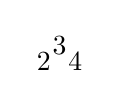
\begin{tikzpicture}[scale=0.2]
								\node at (-1,-1){$2$};
								\node at (0,0){$3$};
								\node at (1,-1){$4$};
					\end{tikzpicture}}};
					\node (4) at (0,-2){\scalebox{.7}{
							\begin{tikzpicture}[scale=0.2]
								\node at (0,0){$4$};
					\end{tikzpicture}}};
					\node (14) at (2,0){\scalebox{.7}{
							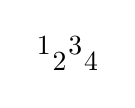
\begin{tikzpicture}[scale=0.2]
								\node at (-2,0){$1$};
								\node at (-1,-1){$2$};
								\node at (0,0){$3$};
								\node at (1,-1){$4$};
					\end{tikzpicture}}};
					\node (23) at (2,-2){\scalebox{.7}{
							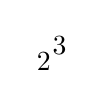
\begin{tikzpicture}[scale=0.2]
								\node at (-1,-1){$2$};
								\node at (0,0){$3$};
					\end{tikzpicture}}};
					\node (34) at (3,1){\scalebox{.7}{
							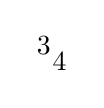
\begin{tikzpicture}[scale=0.2]
								\node at (0,0){$3$};
								\node at (1,-1){$4$};
					\end{tikzpicture}}};
					\node (13) at (3,-1){\scalebox{.7}{
							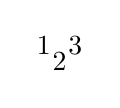
\begin{tikzpicture}[scale=0.2]
								\node at (-1,1){$1$};
								\node at (0,0){$2$};
								\node at (1,1){$3$};
					\end{tikzpicture}}};
					\node (3) at (4,0){\scalebox{.7}{
							\begin{tikzpicture}[scale=0.2]
								\node at (0,0){$3$};
					\end{tikzpicture}}};
					\node (1) at (4,-2){\scalebox{.7}{
							\begin{tikzpicture}[scale=0.2]
								\node at (0,0){$1$};
					\end{tikzpicture}}};
					\draw (2) -- (12);
					\draw (2) -- (24);
					\draw (4) -- (24);
					\draw (12) -- (14);
					\draw (24) -- (14);
					\draw (24) -- (23);
					\draw (14) -- (34);
					\draw (14) -- (13);
					\draw (23) -- (13);
					\draw (34) -- (3);
					\draw (13) -- (3);
					\draw (13) -- (1);
				\end{scope}
				\begin{scope}[xshift=5cm, yshift = 0cm,line width=.5mm,scale=.85]
					\node at (1,1.5){Tilting modules};
					\node (a) at (0,0){\scalebox{.35}{\begin{tikzpicture}[line width=.3mm, ->, >= angle 60]
								\node[rectangle,line width=0mm,fill=bleudefrance!10,draw] (2) at (0,0){\scalebox{.7}{
										\begin{tikzpicture}[scale=0.2]
											\node at (0,0){$2$};
								\end{tikzpicture}}};
								\node[rectangle,line width=0mm,fill=bleudefrance!10,draw] (12) at (1,1){\scalebox{.7}{
										\begin{tikzpicture}[scale=0.2]
											\node at (0,0){$1$};
											\node at (1,-1){$2$};
								\end{tikzpicture}}};
								\node[rectangle,line width=0mm,fill=bleudefrance!10,draw] (24) at (1,-1){\scalebox{.7}{
										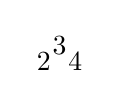
\begin{tikzpicture}[scale=0.2]
											\node at (-1,-1){$2$};
											\node at (0,0){$3$};
											\node at (1,-1){$4$};
								\end{tikzpicture}}};
								\node (4) at (0,-2)[rectangle,line width=0mm,fill=bleudefrance!10,draw]{\scalebox{.7}{
										\begin{tikzpicture}[scale=0.2]
											\node at (0,0){$4$};
								\end{tikzpicture}}};
								\node (14) at (2,0){\scalebox{.7}{
										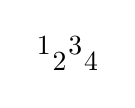
\begin{tikzpicture}[scale=0.2]
											\node at (-2,0){$1$};
											\node at (-1,-1){$2$};
											\node at (0,0){$3$};
											\node at (1,-1){$4$};
								\end{tikzpicture}}};
								\node (23) at (2,-2){\scalebox{.7}{
										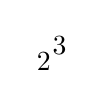
\begin{tikzpicture}[scale=0.2]
											\node at (-1,-1){$2$};
											\node at (0,0){$3$};
								\end{tikzpicture}}};
								\node (34) at (3,1){\scalebox{.7}{
										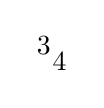
\begin{tikzpicture}[scale=0.2]
											\node at (0,0){$3$};
											\node at (1,-1){$4$};
								\end{tikzpicture}}};
								\node (13) at (3,-1){\scalebox{.7}{
										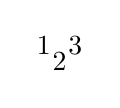
\begin{tikzpicture}[scale=0.2]
											\node at (-1,1){$1$};
											\node at (0,0){$2$};
											\node at (1,1){$3$};
								\end{tikzpicture}}};
								\node (3) at (4,0){\scalebox{.7}{
										\begin{tikzpicture}[scale=0.2]
											\node at (0,0){$3$};
								\end{tikzpicture}}};
								\node (1) at (4,-2){\scalebox{.7}{
										\begin{tikzpicture}[scale=0.2]
											\node at (0,0){$1$};
								\end{tikzpicture}}};
								\draw (2) -- (12);
								\draw (2) -- (24);
								\draw (4) -- (24);
								\draw (12) -- (14);
								\draw (24) -- (14);
								\draw (24) -- (23);
								\draw (14) -- (34);
								\draw (14) -- (13);
								\draw (23) -- (13);
								\draw (34) -- (3);
								\draw (13) -- (3);
								\draw (13) -- (1);
					\end{tikzpicture}}};
					\node (b) at (2,0){\scalebox{.35}{\begin{tikzpicture}[line width=.3mm, ->, >= angle 60]
								\node (2) at (0,0){\scalebox{.7}{
										\begin{tikzpicture}[scale=0.2]
											\node at (0,0){$2$};
								\end{tikzpicture}}};
								\node[rectangle,line width=0mm,fill=bleudefrance!10,draw] (12) at (1,1){\scalebox{.7}{
										\begin{tikzpicture}[scale=0.2]
											\node at (0,0){$1$};
											\node at (1,-1){$2$};
								\end{tikzpicture}}};
								\node[rectangle,line width=0mm,fill=bleudefrance!10,draw] (24) at (1,-1){\scalebox{.7}{
										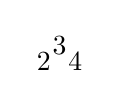
\begin{tikzpicture}[scale=0.2]
											\node at (-1,-1){$2$};
											\node at (0,0){$3$};
											\node at (1,-1){$4$};
								\end{tikzpicture}}};
								\node[rectangle,line width=0mm,fill=bleudefrance!10,draw](4) at (0,-2){\scalebox{.7}{
										\begin{tikzpicture}[scale=0.2]
											\node at (0,0){$4$};
								\end{tikzpicture}}};
								\node[rectangle,line width=0mm,fill=bleudefrance!10,draw] (14) at (2,0){\scalebox{.7}{
										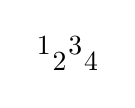
\begin{tikzpicture}[scale=0.2]
											\node at (-2,0){$1$};
											\node at (-1,-1){$2$};
											\node at (0,0){$3$};
											\node at (1,-1){$4$};
								\end{tikzpicture}}};
								\node (23) at (2,-2){\scalebox{.7}{
										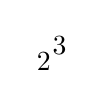
\begin{tikzpicture}[scale=0.2]
											\node at (-1,-1){$2$};
											\node at (0,0){$3$};
								\end{tikzpicture}}};
								\node (34) at (3,1){\scalebox{.7}{
										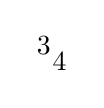
\begin{tikzpicture}[scale=0.2]
											\node at (0,0){$3$};
											\node at (1,-1){$4$};
								\end{tikzpicture}}};
								\node (13) at (3,-1){\scalebox{.7}{
										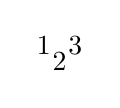
\begin{tikzpicture}[scale=0.2]
											\node at (-1,1){$1$};
											\node at (0,0){$2$};
											\node at (1,1){$3$};
								\end{tikzpicture}}};
								\node (3) at (4,0){\scalebox{.7}{
										\begin{tikzpicture}[scale=0.2]
											\node at (0,0){$3$};
								\end{tikzpicture}}};
								\node (1) at (4,-2){\scalebox{.7}{
										\begin{tikzpicture}[scale=0.2]
											\node at (0,0){$1$};
								\end{tikzpicture}}};
								\draw (2) -- (12);
								\draw (2) -- (24);
								\draw (4) -- (24);
								\draw (12) -- (14);
								\draw (24) -- (14);
								\draw (24) -- (23);
								\draw (14) -- (34);
								\draw (14) -- (13);
								\draw (23) -- (13);
								\draw (34) -- (3);
								\draw (13) -- (3);
								\draw (13) -- (1);
					\end{tikzpicture}}};
					\node (c) at (4,0){\scalebox{.35}{\begin{tikzpicture}[line width=.3mm, ->, >= angle 60]
								\node[rectangle,line width=0mm,fill=bleudefrance!10,draw] (2) at (0,0){\scalebox{.7}{
										\begin{tikzpicture}[scale=0.2]
											\node at (0,0){$2$};
								\end{tikzpicture}}};
								\node[rectangle,line width=0mm,fill=bleudefrance!10,draw] (12) at (1,1){\scalebox{.7}{
										\begin{tikzpicture}[scale=0.2]
											\node at (0,0){$1$};
											\node at (1,-1){$2$};
								\end{tikzpicture}}};
								\node[rectangle,line width=0mm,fill=bleudefrance!10,draw] (24) at (1,-1){\scalebox{.7}{
										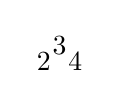
\begin{tikzpicture}[scale=0.2]
											\node at (-1,-1){$2$};
											\node at (0,0){$3$};
											\node at (1,-1){$4$};
								\end{tikzpicture}}};
								\node(4) at (0,-2){\scalebox{.7}{
										\begin{tikzpicture}[scale=0.2]
											\node at (0,0){$4$};
								\end{tikzpicture}}};
								\node (14) at (2,0){\scalebox{.7}{
										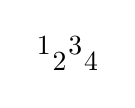
\begin{tikzpicture}[scale=0.2]
											\node at (-2,0){$1$};
											\node at (-1,-1){$2$};
											\node at (0,0){$3$};
											\node at (1,-1){$4$};
								\end{tikzpicture}}};
								\node[rectangle,line width=0mm,fill=bleudefrance!10,draw] (23) at (2,-2){\scalebox{.7}{
										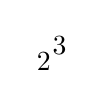
\begin{tikzpicture}[scale=0.2]
											\node at (-1,-1){$2$};
											\node at (0,0){$3$};
								\end{tikzpicture}}};
								\node (34) at (3,1){\scalebox{.7}{
										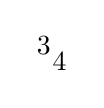
\begin{tikzpicture}[scale=0.2]
											\node at (0,0){$3$};
											\node at (1,-1){$4$};
								\end{tikzpicture}}};
								\node (13) at (3,-1){\scalebox{.7}{
										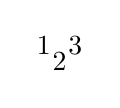
\begin{tikzpicture}[scale=0.2]
											\node at (-1,1){$1$};
											\node at (0,0){$2$};
											\node at (1,1){$3$};
								\end{tikzpicture}}};
								\node (3) at (4,0){\scalebox{.7}{
										\begin{tikzpicture}[scale=0.2]
											\node at (0,0){$3$};
								\end{tikzpicture}}};
								\node (1) at (4,-2){\scalebox{.7}{
										\begin{tikzpicture}[scale=0.2]
											\node at (0,0){$1$};
								\end{tikzpicture}}};
								\draw (2) -- (12);
								\draw (2) -- (24);
								\draw (4) -- (24);
								\draw (12) -- (14);
								\draw (24) -- (14);
								\draw (24) -- (23);
								\draw (14) -- (34);
								\draw (14) -- (13);
								\draw (23) -- (13);
								\draw (34) -- (3);
								\draw (13) -- (3);
								\draw (13) -- (1);
					\end{tikzpicture}}};
					\node (d) at (6,0){\scalebox{.35}{\begin{tikzpicture}[line width=.3mm, ->, >= angle 60]
								\node (2) at (0,0){\scalebox{.7}{
										\begin{tikzpicture}[scale=0.2]
											\node at (0,0){$2$};
								\end{tikzpicture}}};
								\node[rectangle,line width=0mm,fill=bleudefrance!10,draw] (12) at (1,1){\scalebox{.7}{
										\begin{tikzpicture}[scale=0.2]
											\node at (0,0){$1$};
											\node at (1,-1){$2$};
								\end{tikzpicture}}};
								\node[rectangle,line width=0mm,fill=bleudefrance!10,draw] (24) at (1,-1){\scalebox{.7}{
										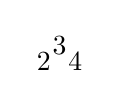
\begin{tikzpicture}[scale=0.2]
											\node at (-1,-1){$2$};
											\node at (0,0){$3$};
											\node at (1,-1){$4$};
								\end{tikzpicture}}};
								\node(4) at (0,-2){\scalebox{.7}{
										\begin{tikzpicture}[scale=0.2]
											\node at (0,0){$4$};
								\end{tikzpicture}}};
								\node[rectangle,line width=0mm,fill=bleudefrance!10,draw] (14) at (2,0){\scalebox{.7}{
										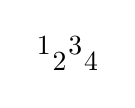
\begin{tikzpicture}[scale=0.2]
											\node at (-2,0){$1$};
											\node at (-1,-1){$2$};
											\node at (0,0){$3$};
											\node at (1,-1){$4$};
								\end{tikzpicture}}};
								\node[rectangle,line width=0mm,fill=bleudefrance!10,draw] (23) at (2,-2){\scalebox{.7}{
										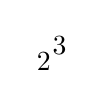
\begin{tikzpicture}[scale=0.2]
											\node at (-1,-1){$2$};
											\node at (0,0){$3$};
								\end{tikzpicture}}};
								\node (34) at (3,1){\scalebox{.7}{
										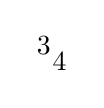
\begin{tikzpicture}[scale=0.2]
											\node at (0,0){$3$};
											\node at (1,-1){$4$};
								\end{tikzpicture}}};
								\node (13) at (3,-1){\scalebox{.7}{
										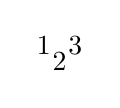
\begin{tikzpicture}[scale=0.2]
											\node at (-1,1){$1$};
											\node at (0,0){$2$};
											\node at (1,1){$3$};
								\end{tikzpicture}}};
								\node (3) at (4,0){\scalebox{.7}{
										\begin{tikzpicture}[scale=0.2]
											\node at (0,0){$3$};
								\end{tikzpicture}}};
								\node (1) at (4,-2){\scalebox{.7}{
										\begin{tikzpicture}[scale=0.2]
											\node at (0,0){$1$};
								\end{tikzpicture}}};
								\draw (2) -- (12);
								\draw (2) -- (24);
								\draw (4) -- (24);
								\draw (12) -- (14);
								\draw (24) -- (14);
								\draw (24) -- (23);
								\draw (14) -- (34);
								\draw (14) -- (13);
								\draw (23) -- (13);
								\draw (34) -- (3);
								\draw (13) -- (3);
								\draw (13) -- (1);
					\end{tikzpicture}}};
					\node (e) at (0,-2){\scalebox{.35}{\begin{tikzpicture}[line width=.3mm, ->, >= angle 60]
								\node (2) at (0,0){\scalebox{.7}{
										\begin{tikzpicture}[scale=0.2]
											\node at (0,0){$2$};
								\end{tikzpicture}}};
								\node (12) at (1,1){\scalebox{.7}{
										\begin{tikzpicture}[scale=0.2]
											\node at (0,0){$1$};
											\node at (1,-1){$2$};
								\end{tikzpicture}}};
								\node[rectangle,line width=0mm,fill=bleudefrance!10,draw] (24) at (1,-1){\scalebox{.7}{
										\begin{tikzpicture}[scale=0.2]
											\node at (-1,-1){$2$};
											\node at (0,0){$3$};
											\node at (1,-1){$4$};
								\end{tikzpicture}}};
								\node[rectangle,line width=0mm,fill=bleudefrance!10,draw](4) at (0,-2){\scalebox{.7}{
										\begin{tikzpicture}[scale=0.2]
											\node at (0,0){$4$};
								\end{tikzpicture}}};
								\node[rectangle,line width=0mm,fill=bleudefrance!10,draw] (14) at (2,0){\scalebox{.7}{
										\begin{tikzpicture}[scale=0.2]
											\node at (-2,0){$1$};
											\node at (-1,-1){$2$};
											\node at (0,0){$3$};
											\node at (1,-1){$4$};
								\end{tikzpicture}}};
								\node (23) at (2,-2){\scalebox{.7}{
										\begin{tikzpicture}[scale=0.2]
											\node at (-1,-1){$2$};
											\node at (0,0){$3$};
								\end{tikzpicture}}};
								\node[rectangle,line width=0mm,fill=bleudefrance!10,draw] (34) at (3,1){\scalebox{.7}{
										\begin{tikzpicture}[scale=0.2]
											\node at (0,0){$3$};
											\node at (1,-1){$4$};
								\end{tikzpicture}}};
								\node (13) at (3,-1){\scalebox{.7}{
										\begin{tikzpicture}[scale=0.2]
											\node at (-1,1){$1$};
											\node at (0,0){$2$};
											\node at (1,1){$3$};
								\end{tikzpicture}}};
								\node (3) at (4,0){\scalebox{.7}{
										\begin{tikzpicture}[scale=0.2]
											\node at (0,0){$3$};
								\end{tikzpicture}}};
								\node (1) at (4,-2){\scalebox{.7}{
										\begin{tikzpicture}[scale=0.2]
											\node at (0,0){$1$};
								\end{tikzpicture}}};
								\draw (2) -- (12);
								\draw (2) -- (24);
								\draw (4) -- (24);
								\draw (12) -- (14);
								\draw (24) -- (14);
								\draw (24) -- (23);
								\draw (14) -- (34);
								\draw (14) -- (13);
								\draw (23) -- (13);
								\draw (34) -- (3);
								\draw (13) -- (3);
								\draw (13) -- (1);
					\end{tikzpicture}}};
					\node (f) at (2,-2){\scalebox{.35}{\begin{tikzpicture}[line width=.3mm, ->, >= angle 60]
								\node (2) at (0,0){\scalebox{.7}{
										\begin{tikzpicture}[scale=0.2]
											\node at (0,0){$2$};
								\end{tikzpicture}}};
								\node[rectangle,line width=0mm,fill=bleudefrance!10,draw] (12) at (1,1){\scalebox{.7}{
										\begin{tikzpicture}[scale=0.2]
											\node at (0,0){$1$};
											\node at (1,-1){$2$};
								\end{tikzpicture}}};
								\node (24) at (1,-1){\scalebox{.7}{
										\begin{tikzpicture}[scale=0.2]
											\node at (-1,-1){$2$};
											\node at (0,0){$3$};
											\node at (1,-1){$4$};
								\end{tikzpicture}}};
								\node[rectangle,line width=0mm,fill=bleudefrance!10,draw](4) at (0,-2){\scalebox{.7}{
										\begin{tikzpicture}[scale=0.2]
											\node at (0,0){$4$};
								\end{tikzpicture}}};
								\node[rectangle,line width=0mm,fill=bleudefrance!10,draw] (14) at (2,0){\scalebox{.7}{
										\begin{tikzpicture}[scale=0.2]
											\node at (-2,0){$1$};
											\node at (-1,-1){$2$};
											\node at (0,0){$3$};
											\node at (1,-1){$4$};
								\end{tikzpicture}}};
								\node (23) at (2,-2){\scalebox{.7}{
										\begin{tikzpicture}[scale=0.2]
											\node at (-1,-1){$2$};
											\node at (0,0){$3$};
								\end{tikzpicture}}};
								\node (34) at (3,1){\scalebox{.7}{
										\begin{tikzpicture}[scale=0.2]
											\node at (0,0){$3$};
											\node at (1,-1){$4$};
								\end{tikzpicture}}};
								\node (13) at (3,-1){\scalebox{.7}{
										\begin{tikzpicture}[scale=0.2]
											\node at (-1,1){$1$};
											\node at (0,0){$2$};
											\node at (1,1){$3$};
								\end{tikzpicture}}};
								\node (3) at (4,0){\scalebox{.7}{
										\begin{tikzpicture}[scale=0.2]
											\node at (0,0){$3$};
								\end{tikzpicture}}};
								\node[rectangle,line width=0mm,fill=bleudefrance!10,draw] (1) at (4,-2){\scalebox{.7}{
										\begin{tikzpicture}[scale=0.2]
											\node at (0,0){$1$};
								\end{tikzpicture}}};
								\draw (2) -- (12);
								\draw (2) -- (24);
								\draw (4) -- (24);
								\draw (12) -- (14);
								\draw (24) -- (14);
								\draw (24) -- (23);
								\draw (14) -- (34);
								\draw (14) -- (13);
								\draw (23) -- (13);
								\draw (34) -- (3);
								\draw (13) -- (3);
								\draw (13) -- (1);
					\end{tikzpicture}}};
					\node (g) at (4,-2){\scalebox{.35}{\begin{tikzpicture}[line width=.3mm, ->, >= angle 60]
								\node (2) at (0,0){\scalebox{.7}{
										\begin{tikzpicture}[scale=0.2]
											\node at (0,0){$2$};
								\end{tikzpicture}}};
								\node[rectangle,line width=0mm,fill=bleudefrance!10,draw] (12) at (1,1){\scalebox{.7}{
										\begin{tikzpicture}[scale=0.2]
											\node at (0,0){$1$};
											\node at (1,-1){$2$};
								\end{tikzpicture}}};
								\node (24) at (1,-1){\scalebox{.7}{
										\begin{tikzpicture}[scale=0.2]
											\node at (-1,-1){$2$};
											\node at (0,0){$3$};
											\node at (1,-1){$4$};
								\end{tikzpicture}}};
								\node(4) at (0,-2){\scalebox{.7}{
										\begin{tikzpicture}[scale=0.2]
											\node at (0,0){$4$};
								\end{tikzpicture}}};
								\node[rectangle,line width=0mm,fill=bleudefrance!10,draw] (14) at (2,0){\scalebox{.7}{
										\begin{tikzpicture}[scale=0.2]
											\node at (-2,0){$1$};
											\node at (-1,-1){$2$};
											\node at (0,0){$3$};
											\node at (1,-1){$4$};
								\end{tikzpicture}}};
								\node[rectangle,line width=0mm,fill=bleudefrance!10,draw] (23) at (2,-2){\scalebox{.7}{
										\begin{tikzpicture}[scale=0.2]
											\node at (-1,-1){$2$};
											\node at (0,0){$3$};
								\end{tikzpicture}}};
								\node (34) at (3,1){\scalebox{.7}{
										\begin{tikzpicture}[scale=0.2]
											\node at (0,0){$3$};
											\node at (1,-1){$4$};
								\end{tikzpicture}}};
								\node[rectangle,line width=0mm,fill=bleudefrance!10,draw] (13) at (3,-1){\scalebox{.7}{
										\begin{tikzpicture}[scale=0.2]
											\node at (-1,1){$1$};
											\node at (0,0){$2$};
											\node at (1,1){$3$};
								\end{tikzpicture}}};
								\node (3) at (4,0){\scalebox{.7}{
										\begin{tikzpicture}[scale=0.2]
											\node at (0,0){$3$};
								\end{tikzpicture}}};
								\node (1) at (4,-2){\scalebox{.7}{
										\begin{tikzpicture}[scale=0.2]
											\node at (0,0){$1$};
								\end{tikzpicture}}};
								\draw (2) -- (12);
								\draw (2) -- (24);
								\draw (4) -- (24);
								\draw (12) -- (14);
								\draw (24) -- (14);
								\draw (24) -- (23);
								\draw (14) -- (34);
								\draw (14) -- (13);
								\draw (23) -- (13);
								\draw (34) -- (3);
								\draw (13) -- (3);
								\draw (13) -- (1);
					\end{tikzpicture}}};
					\node (h) at (6,-2){\scalebox{.35}{\begin{tikzpicture}[line width=.3mm, ->, >= angle 60]
								\node (2) at (0,0){\scalebox{.7}{
										\begin{tikzpicture}[scale=0.2]
											\node at (0,0){$2$};
								\end{tikzpicture}}};
								\node (12) at (1,1){\scalebox{.7}{
										\begin{tikzpicture}[scale=0.2]
											\node at (0,0){$1$};
											\node at (1,-1){$2$};
								\end{tikzpicture}}};
								\node[rectangle,line width=0mm,fill=bleudefrance!10,draw] (24) at (1,-1){\scalebox{.7}{
										\begin{tikzpicture}[scale=0.2]
											\node at (-1,-1){$2$};
											\node at (0,0){$3$};
											\node at (1,-1){$4$};
								\end{tikzpicture}}};
								\node(4) at (0,-2){\scalebox{.7}{
										\begin{tikzpicture}[scale=0.2]
											\node at (0,0){$4$};
								\end{tikzpicture}}};
								\node[rectangle,line width=0mm,fill=bleudefrance!10,draw] (14) at (2,0){\scalebox{.7}{
										\begin{tikzpicture}[scale=0.2]
											\node at (-2,0){$1$};
											\node at (-1,-1){$2$};
											\node at (0,0){$3$};
											\node at (1,-1){$4$};
								\end{tikzpicture}}};
								\node[rectangle,line width=0mm,fill=bleudefrance!10,draw] (23) at (2,-2){\scalebox{.7}{
										\begin{tikzpicture}[scale=0.2]
											\node at (-1,-1){$2$};
											\node at (0,0){$3$};
								\end{tikzpicture}}};
								\node[rectangle,line width=0mm,fill=bleudefrance!10,draw] (34) at (3,1){\scalebox{.7}{
										\begin{tikzpicture}[scale=0.2]
											\node at (0,0){$3$};
											\node at (1,-1){$4$};
								\end{tikzpicture}}};
								\node (13) at (3,-1){\scalebox{.7}{
										\begin{tikzpicture}[scale=0.2]
											\node at (-1,1){$1$};
											\node at (0,0){$2$};
											\node at (1,1){$3$};
								\end{tikzpicture}}};
								\node (3) at (4,0){\scalebox{.7}{
										\begin{tikzpicture}[scale=0.2]
											\node at (0,0){$3$};
								\end{tikzpicture}}};
								\node (1) at (4,-2){\scalebox{.7}{
										\begin{tikzpicture}[scale=0.2]
											\node at (0,0){$1$};
								\end{tikzpicture}}};
								\draw (2) -- (12);
								\draw (2) -- (24);
								\draw (4) -- (24);
								\draw (12) -- (14);
								\draw (24) -- (14);
								\draw (24) -- (23);
								\draw (14) -- (34);
								\draw (14) -- (13);
								\draw (23) -- (13);
								\draw (34) -- (3);
								\draw (13) -- (3);
								\draw (13) -- (1);
					\end{tikzpicture}}};
					\node (i) at (0,-4){\scalebox{.35}{\begin{tikzpicture}[line width=.3mm, ->, >= angle 60]
								\node (2) at (0,0){\scalebox{.7}{
										\begin{tikzpicture}[scale=0.2]
											\node at (0,0){$2$};
								\end{tikzpicture}}};
								\node (12) at (1,1){\scalebox{.7}{
										\begin{tikzpicture}[scale=0.2]
											\node at (0,0){$1$};
											\node at (1,-1){$2$};
								\end{tikzpicture}}};
								\node (24) at (1,-1){\scalebox{.7}{
										\begin{tikzpicture}[scale=0.2]
											\node at (-1,-1){$2$};
											\node at (0,0){$3$};
											\node at (1,-1){$4$};
								\end{tikzpicture}}};
								\node[rectangle,line width=0mm,fill=bleudefrance!10,draw] (4) at (0,-2){\scalebox{.7}{
										\begin{tikzpicture}[scale=0.2]
											\node at (0,0){$4$};
								\end{tikzpicture}}};
								\node[rectangle,line width=0mm,fill=bleudefrance!10,draw] (14) at (2,0){\scalebox{.7}{
										\begin{tikzpicture}[scale=0.2]
											\node at (-2,0){$1$};
											\node at (-1,-1){$2$};
											\node at (0,0){$3$};
											\node at (1,-1){$4$};
								\end{tikzpicture}}};
								\node (23) at (2,-2){\scalebox{.7}{
										\begin{tikzpicture}[scale=0.2]
											\node at (-1,-1){$2$};
											\node at (0,0){$3$};
								\end{tikzpicture}}};
								\node[rectangle,line width=0mm,fill=bleudefrance!10,draw] (34) at (3,1){\scalebox{.7}{
										\begin{tikzpicture}[scale=0.2]
											\node at (0,0){$3$};
											\node at (1,-1){$4$};
								\end{tikzpicture}}};
								\node (13) at (3,-1){\scalebox{.7}{
										\begin{tikzpicture}[scale=0.2]
											\node at (-1,1){$1$};
											\node at (0,0){$2$};
											\node at (1,1){$3$};
								\end{tikzpicture}}};
								\node (3) at (4,0){\scalebox{.7}{
										\begin{tikzpicture}[scale=0.2]
											\node at (0,0){$3$};
								\end{tikzpicture}}};
								\node[rectangle,line width=0mm,fill=bleudefrance!10,draw] (1) at (4,-2){\scalebox{.7}{
										\begin{tikzpicture}[scale=0.2]
											\node at (0,0){$1$};
								\end{tikzpicture}}};
								\draw (2) -- (12);
								\draw (2) -- (24);
								\draw (4) -- (24);
								\draw (12) -- (14);
								\draw (24) -- (14);
								\draw (24) -- (23);
								\draw (14) -- (34);
								\draw (14) -- (13);
								\draw (23) -- (13);
								\draw (34) -- (3);
								\draw (13) -- (3);
								\draw (13) -- (1);
					\end{tikzpicture}}};
					\node (j) at (2,-4){\scalebox{.35}{\begin{tikzpicture}[line width=.3mm, ->, >= angle 60]
								\node (2) at (0,0){\scalebox{.7}{
										\begin{tikzpicture}[scale=0.2]
											\node at (0,0){$2$};
								\end{tikzpicture}}};
								\node[rectangle,line width=0mm,fill=bleudefrance!10,draw] (12) at (1,1){\scalebox{.7}{
										\begin{tikzpicture}[scale=0.2]
											\node at (0,0){$1$};
											\node at (1,-1){$2$};
								\end{tikzpicture}}};
								\node (24) at (1,-1){\scalebox{.7}{
										\begin{tikzpicture}[scale=0.2]
											\node at (-1,-1){$2$};
											\node at (0,0){$3$};
											\node at (1,-1){$4$};
								\end{tikzpicture}}};
								\node(4) at (0,-2){\scalebox{.7}{
										\begin{tikzpicture}[scale=0.2]
											\node at (0,0){$4$};
								\end{tikzpicture}}};
								\node[rectangle,line width=0mm,fill=bleudefrance!10,draw] (14) at (2,0){\scalebox{.7}{
										\begin{tikzpicture}[scale=0.2]
											\node at (-2,0){$1$};
											\node at (-1,-1){$2$};
											\node at (0,0){$3$};
											\node at (1,-1){$4$};
								\end{tikzpicture}}};
								\node (23) at (2,-2){\scalebox{.7}{
										\begin{tikzpicture}[scale=0.2]
											\node at (-1,-1){$2$};
											\node at (0,0){$3$};
								\end{tikzpicture}}};
								\node (34) at (3,1){\scalebox{.7}{
										\begin{tikzpicture}[scale=0.2]
											\node at (0,0){$3$};
											\node at (1,-1){$4$};
								\end{tikzpicture}}};
								\node[rectangle,line width=0mm,fill=bleudefrance!10,draw] (13) at (3,-1){\scalebox{.7}{
										\begin{tikzpicture}[scale=0.2]
											\node at (-1,1){$1$};
											\node at (0,0){$2$};
											\node at (1,1){$3$};
								\end{tikzpicture}}};
								\node (3) at (4,0){\scalebox{.7}{
										\begin{tikzpicture}[scale=0.2]
											\node at (0,0){$3$};
								\end{tikzpicture}}};
								\node[rectangle,line width=0mm,fill=bleudefrance!10,draw] (1) at (4,-2){\scalebox{.7}{
										\begin{tikzpicture}[scale=0.2]
											\node at (0,0){$1$};
								\end{tikzpicture}}};
								\draw (2) -- (12);
								\draw (2) -- (24);
								\draw (4) -- (24);
								\draw (12) -- (14);
								\draw (24) -- (14);
								\draw (24) -- (23);
								\draw (14) -- (34);
								\draw (14) -- (13);
								\draw (23) -- (13);
								\draw (34) -- (3);
								\draw (13) -- (3);
								\draw (13) -- (1);
					\end{tikzpicture}}};
					\node (k) at (4,-4){\scalebox{.35}{\begin{tikzpicture}[line width=.3mm, ->, >= angle 60]
								\node (2) at (0,0){\scalebox{.7}{
										\begin{tikzpicture}[scale=0.2]
											\node at (0,0){$2$};
								\end{tikzpicture}}};
								\node (12) at (1,1){\scalebox{.7}{
										\begin{tikzpicture}[scale=0.2]
											\node at (0,0){$1$};
											\node at (1,-1){$2$};
								\end{tikzpicture}}};
								\node (24) at (1,-1){\scalebox{.7}{
										\begin{tikzpicture}[scale=0.2]
											\node at (-1,-1){$2$};
											\node at (0,0){$3$};
											\node at (1,-1){$4$};
								\end{tikzpicture}}};
								\node(4) at (0,-2){\scalebox{.7}{
										\begin{tikzpicture}[scale=0.2]
											\node at (0,0){$4$};
								\end{tikzpicture}}};
								\node[rectangle,line width=0mm,fill=bleudefrance!10,draw] (14) at (2,0){\scalebox{.7}{
										\begin{tikzpicture}[scale=0.2]
											\node at (-2,0){$1$};
											\node at (-1,-1){$2$};
											\node at (0,0){$3$};
											\node at (1,-1){$4$};
								\end{tikzpicture}}};
								\node[rectangle,line width=0mm,fill=bleudefrance!10,draw] (23) at (2,-2){\scalebox{.7}{
										\begin{tikzpicture}[scale=0.2]
											\node at (-1,-1){$2$};
											\node at (0,0){$3$};
								\end{tikzpicture}}};
								\node[rectangle,line width=0mm,fill=bleudefrance!10,draw] (34) at (3,1){\scalebox{.7}{
										\begin{tikzpicture}[scale=0.2]
											\node at (0,0){$3$};
											\node at (1,-1){$4$};
								\end{tikzpicture}}};
								\node[rectangle,line width=0mm,fill=bleudefrance!10,draw] (13) at (3,-1){\scalebox{.7}{
										\begin{tikzpicture}[scale=0.2]
											\node at (-1,1){$1$};
											\node at (0,0){$2$};
											\node at (1,1){$3$};
								\end{tikzpicture}}};
								\node (3) at (4,0){\scalebox{.7}{
										\begin{tikzpicture}[scale=0.2]
											\node at (0,0){$3$};
								\end{tikzpicture}}};
								\node (1) at (4,-2){\scalebox{.7}{
										\begin{tikzpicture}[scale=0.2]
											\node at (0,0){$1$};
								\end{tikzpicture}}};
								\draw (2) -- (12);
								\draw (2) -- (24);
								\draw (4) -- (24);
								\draw (12) -- (14);
								\draw (24) -- (14);
								\draw (24) -- (23);
								\draw (14) -- (34);
								\draw (14) -- (13);
								\draw (23) -- (13);
								\draw (34) -- (3);
								\draw (13) -- (3);
								\draw (13) -- (1);
					\end{tikzpicture}}};
					\node (l) at (6,-4){\scalebox{.35}{\begin{tikzpicture}[line width=.3mm, ->, >= angle 60]
								\node (2) at (0,0){\scalebox{.7}{
										\begin{tikzpicture}[scale=0.2]
											\node at (0,0){$2$};
								\end{tikzpicture}}};
								\node (12) at (1,1){\scalebox{.7}{
										\begin{tikzpicture}[scale=0.2]
											\node at (0,0){$1$};
											\node at (1,-1){$2$};
								\end{tikzpicture}}};
								\node (24) at (1,-1){\scalebox{.7}{
										\begin{tikzpicture}[scale=0.2]
											\node at (-1,-1){$2$};
											\node at (0,0){$3$};
											\node at (1,-1){$4$};
								\end{tikzpicture}}};
								\node(4) at (0,-2){\scalebox{.7}{
										\begin{tikzpicture}[scale=0.2]
											\node at (0,0){$4$};
								\end{tikzpicture}}};
								\node[rectangle,line width=0mm,fill=bleudefrance!10,draw] (14) at (2,0){\scalebox{.7}{
										\begin{tikzpicture}[scale=0.2]
											\node at (-2,0){$1$};
											\node at (-1,-1){$2$};
											\node at (0,0){$3$};
											\node at (1,-1){$4$};
								\end{tikzpicture}}};
								\node (23) at (2,-2){\scalebox{.7}{
										\begin{tikzpicture}[scale=0.2]
											\node at (-1,-1){$2$};
											\node at (0,0){$3$};
								\end{tikzpicture}}};
								\node[rectangle,line width=0mm,fill=bleudefrance!10,draw] (34) at (3,1){\scalebox{.7}{
										\begin{tikzpicture}[scale=0.2]
											\node at (0,0){$3$};
											\node at (1,-1){$4$};
								\end{tikzpicture}}};
								\node[rectangle,line width=0mm,fill=bleudefrance!10,draw] (13) at (3,-1){\scalebox{.7}{
										\begin{tikzpicture}[scale=0.2]
											\node at (-1,1){$1$};
											\node at (0,0){$2$};
											\node at (1,1){$3$};
								\end{tikzpicture}}};
								\node (3) at (4,0){\scalebox{.7}{
										\begin{tikzpicture}[scale=0.2]
											\node at (0,0){$3$};
								\end{tikzpicture}}};
								\node[rectangle,line width=0mm,fill=bleudefrance!10,draw] (1) at (4,-2){\scalebox{.7}{
										\begin{tikzpicture}[scale=0.2]
											\node at (0,0){$1$};
								\end{tikzpicture}}};
								\draw (2) -- (12);
								\draw (2) -- (24);
								\draw (4) -- (24);
								\draw (12) -- (14);
								\draw (24) -- (14);
								\draw (24) -- (23);
								\draw (14) -- (34);
								\draw (14) -- (13);
								\draw (23) -- (13);
								\draw (34) -- (3);
								\draw (13) -- (3);
								\draw (13) -- (1);
					\end{tikzpicture}}};
					\node (m) at (2,-6){\scalebox{.35}{\begin{tikzpicture}[line width=.3mm, ->, >= angle 60]
								\node (2) at (0,0){\scalebox{.7}{
										\begin{tikzpicture}[scale=0.2]
											\node at (0,0){$2$};
								\end{tikzpicture}}};
								\node (12) at (1,1){\scalebox{.7}{
										\begin{tikzpicture}[scale=0.2]
											\node at (0,0){$1$};
											\node at (1,-1){$2$};
								\end{tikzpicture}}};
								\node (24) at (1,-1){\scalebox{.7}{
										\begin{tikzpicture}[scale=0.2]
											\node at (-1,-1){$2$};
											\node at (0,0){$3$};
											\node at (1,-1){$4$};
								\end{tikzpicture}}};
								\node(4) at (0,-2){\scalebox{.7}{
										\begin{tikzpicture}[scale=0.2]
											\node at (0,0){$4$};
								\end{tikzpicture}}};
								\node (14) at (2,0){\scalebox{.7}{
										\begin{tikzpicture}[scale=0.2]
											\node at (-2,0){$1$};
											\node at (-1,-1){$2$};
											\node at (0,0){$3$};
											\node at (1,-1){$4$};
								\end{tikzpicture}}};
								\node[rectangle,line width=0mm,fill=bleudefrance!10,draw] (23) at (2,-2){\scalebox{.7}{
										\begin{tikzpicture}[scale=0.2]
											\node at (-1,-1){$2$};
											\node at (0,0){$3$};
								\end{tikzpicture}}};
								\node[rectangle,line width=0mm,fill=bleudefrance!10,draw] (34) at (3,1){\scalebox{.7}{
										\begin{tikzpicture}[scale=0.2]
											\node at (0,0){$3$};
											\node at (1,-1){$4$};
								\end{tikzpicture}}};
								\node[rectangle,line width=0mm,fill=bleudefrance!10,draw] (13) at (3,-1){\scalebox{.7}{
										\begin{tikzpicture}[scale=0.2]
											\node at (-1,1){$1$};
											\node at (0,0){$2$};
											\node at (1,1){$3$};
								\end{tikzpicture}}};
								\node[rectangle,line width=0mm,fill=bleudefrance!10,draw] (3) at (4,0){\scalebox{.7}{
										\begin{tikzpicture}[scale=0.2]
											\node at (0,0){$3$};
								\end{tikzpicture}}};
								\node (1) at (4,-2){\scalebox{.7}{
										\begin{tikzpicture}[scale=0.2]
											\node at (0,0){$1$};
								\end{tikzpicture}}};
								\draw (2) -- (12);
								\draw (2) -- (24);
								\draw (4) -- (24);
								\draw (12) -- (14);
								\draw (24) -- (14);
								\draw (24) -- (23);
								\draw (14) -- (34);
								\draw (14) -- (13);
								\draw (23) -- (13);
								\draw (34) -- (3);
								\draw (13) -- (3);
								\draw (13) -- (1);
					\end{tikzpicture}}};
					\node (n) at (4,-6){\scalebox{.35}{\begin{tikzpicture}[line width=.3mm, ->, >= angle 60]
								\node (2) at (0,0){\scalebox{.7}{
										\begin{tikzpicture}[scale=0.2]
											\node at (0,0){$2$};
								\end{tikzpicture}}};
								\node (12) at (1,1){\scalebox{.7}{
										\begin{tikzpicture}[scale=0.2]
											\node at (0,0){$1$};
											\node at (1,-1){$2$};
								\end{tikzpicture}}};
								\node (24) at (1,-1){\scalebox{.7}{
										\begin{tikzpicture}[scale=0.2]
											\node at (-1,-1){$2$};
											\node at (0,0){$3$};
											\node at (1,-1){$4$};
								\end{tikzpicture}}};
								\node(4) at (0,-2){\scalebox{.7}{
										\begin{tikzpicture}[scale=0.2]
											\node at (0,0){$4$};
								\end{tikzpicture}}};
								\node (14) at (2,0){\scalebox{.7}{
										\begin{tikzpicture}[scale=0.2]
											\node at (-2,0){$1$};
											\node at (-1,-1){$2$};
											\node at (0,0){$3$};
											\node at (1,-1){$4$};
								\end{tikzpicture}}};
								\node (23) at (2,-2){\scalebox{.7}{
										\begin{tikzpicture}[scale=0.2]
											\node at (-1,-1){$2$};
											\node at (0,0){$3$};
								\end{tikzpicture}}};
								\node[rectangle,line width=0mm,fill=bleudefrance!10,draw] (34) at (3,1){\scalebox{.7}{
										\begin{tikzpicture}[scale=0.2]
											\node at (0,0){$3$};
											\node at (1,-1){$4$};
								\end{tikzpicture}}};
								\node[rectangle,line width=0mm,fill=bleudefrance!10,draw] (13) at (3,-1){\scalebox{.7}{
										\begin{tikzpicture}[scale=0.2]
											\node at (-1,1){$1$};
											\node at (0,0){$2$};
											\node at (1,1){$3$};
								\end{tikzpicture}}};
								\node[rectangle,line width=0mm,fill=bleudefrance!10,draw] (3) at (4,0){\scalebox{.7}{
										\begin{tikzpicture}[scale=0.2]
											\node at (0,0){$3$};
								\end{tikzpicture}}};
								\node[rectangle,line width=0mm,fill=bleudefrance!10,draw] (1) at (4,-2){\scalebox{.7}{
										\begin{tikzpicture}[scale=0.2]
											\node at (0,0){$1$};
								\end{tikzpicture}}};
								\draw (2) -- (12);
								\draw (2) -- (24);
								\draw (4) -- (24);
								\draw (12) -- (14);
								\draw (24) -- (14);
								\draw (24) -- (23);
								\draw (14) -- (34);
								\draw (14) -- (13);
								\draw (23) -- (13);
								\draw (34) -- (3);
								\draw (13) -- (3);
								\draw (13) -- (1);
					\end{tikzpicture}}};
				\end{scope}
			\end{tikzpicture}
        \caption{Caption}
        \label{fig:enter-label}
    \end{figure}
\end{ex}


\begin{prop}
\label{prop:Tstable}
Let $T,T' \in \Tilt(Q)$. If $T' \in [T]_{\approx_{\mathcal{E}}}$, then $\GS_{\mathcal{E}}(T') = \GS_{\mathcal{E}}(T)$.
\end{prop}
\ibenj{J'ai noté que cette proposition tient également pour n'importe quelle structure exacte.}

\begin{proof}
Let us prove this proposition, it is enough to show that $\GS_{\mathcal{E}}(T') = \GS_{\mathcal{E}}(T)$ whenever $T' \cong \pmb{\mu}_{U,\mathcal{E}}(T)$ for some $U \in \ind(Q)$. We get the desired result by an induction on the length of the sequence of $\mathcal{E}$-mutations that allows us to have $T'\approx_{\mathcal{E}} T$.

We have three cases to treat.
\begin{enumerate}[label=$\bullet$, itemsep=1mm]
    \item If $\pmb{\mu}_{U,\mathcal{E}}(T) \cong T$, then the result is obvious.
    \item If $\pmb{\mu}_{U,\mathcal{E}}(T) = \pmb{\mu}_{U,\mathcal{E}}^-(T)$, by writing $T = \widetilde{T} \oplus U$, we have the following short $\mathcal{E}$-exact sequence: 
\[\begin{tikzcd}
	0 & U & \Theta  & \Coker(f)&  0,
	\arrow[from=1-1, to=1-2]
	\arrow["f",tail, from=1-2, to=1-3]
	\arrow[two heads,from=1-3, to=1-4]
	\arrow[from=1-4, to=1-5]
\end{tikzcd} \] where $f$ is a left minimal $(\add(\widetilde{T}), \mathcal{E})$-approximation of $U$. As $\Theta \in \add(T) \subset \GS_\mathcal{E}(T)$, and $f$ is an $\mathcal{E}$-monomorphism, by \cref{lem:proponGS}, we have that $\Coker(f) \in  \GS_{\mathcal{E}}(T)$. Therefore $T' \cong \widetilde{T} \oplus \Coker(f) \in \GS_{\mathcal{E}}(T)$. 
    \item If $\pmb{\mu}_{U,\mathcal{E}}(T) = \pmb{\mu}_{U, \mathcal{E}}^{+}(X)$, by writing $T = \widetilde{T} \oplus U$, we have the following short $\mathcal{E}$-exact sequence: 
\[\begin{tikzcd}
	0 & \Ker(f) & \Theta' & U &  0,
	\arrow[from=1-1, to=1-2]
	\arrow[tail, from=1-2, to=1-3]
	\arrow["g",two heads,from=1-3, to=1-4]
	\arrow[from=1-4, to=1-5]
\end{tikzcd} \] where $g$ is a right minimal $(\add(\widetilde{T}), \mathcal{E})$-approximation of $U$. As $\Theta' \in \add(\widetilde{T})$ and $g$ is an $\mathcal{E}$-epimorphism, by \cref{lem:proponGS}, we have that $\Ker(f) \in \GS_{\mathcal{E}}(T)$. So $T' \cong \widetilde{T} \oplus \Ker(f) \in \GS_{\mathcal{E}}(T)$.
\end{enumerate}
In either case, we got that $T' \sim_{\mathcal{E}} T$.
\end{proof}

\cref{prop:Tstable} shows that the image of any $T \in \Tilt(Q)$ by $\GS_{\mathcal{E}}$ depends on the equivalent class $[T]_{\approx_{\mathcal{E}}}$. In the case where $\mathcal{E} = \mathcal{E}_\diamond$, we will prove that $\approx_{\mathcal{E}_\diamond}$ and $\sim_{\mathcal{E}_\diamond}$ are the same equivalence relation.

\begin{lemma}[\cite{APT15}] \label{lem:Ibra} 
    Let $T \in \Tilt(Q)$ and $X \in \Gen(T)$. Given a right $\add(T)$-approximation of $X$ \benj{Tu utilise ici le fait que $g$ est un épimorphisme là, non ?}\[\begin{tikzcd}
	\xi : 0 & K & T_0  & X &  0,
	\arrow[from=1-1, to=1-2]
	\arrow[tail, from=1-2, to=1-3]
	\arrow["g",two heads,from=1-3, to=1-4]
	\arrow[from=1-4, to=1-5]
    \end{tikzcd} \]
    then $K \in \add(T)$. Dually, it holds for $\Sub(T)$ and left approximations.
\end{lemma}
\ibenj{Je pense qu'il faudra l'énoncé autrement.}

\begin{lemma} \label{lem:crucialTreaching}
    Let $T \in \Tilt(Q)$ and $X \in \ind(Q)$. If $X \in \GS_\mathcal{E}^1(T)$, then $X \in \add(T)$ or $X \in \add(\pmb{\mu}_{U,\mathcal{E}}(T))$ for some indecomposable summand $U$ in $T$
\end{lemma}

%\ibenj{Je laisse l'énoncé sur n'importe quel structure exact, mais si besoin, il est suffisant de le faire avec $\mathcal{E}_\diamond$.}

\begin{proof}
    Recall that $Q$ is an $A_n$ type quiver. We can easily check this property for $n \leqslant 2$. Let us assume that $X \in \GS_\mathcal{E}^1(T)$. If $X \in \add(T)$, the result occurs. Assume that $X \notin \add(T)$. So $X \in \Gen_\mathcal{E}(T)$ or $X \in \Sub_\mathcal{E}(T)$. In the following, we assume that $X \in \Gen_\mathcal{E}(T)$; the other case can be treated dually.

    There exists a short $\mathcal{E}$-exact sequence
    \[\begin{tikzcd}
	\xi : 0 & Y & \Theta  & X &  0,
	\arrow[from=1-1, to=1-2]
	\arrow[tail, from=1-2, to=1-3]
	\arrow["g",two heads,from=1-3, to=1-4]
	\arrow[from=1-4, to=1-5]
    \end{tikzcd} \] where $\Theta \in \add(T)$. 

As $g$ is an $\mathcal{E}$-epimorphism, \Sunny{Cela n'est pas vrai} then $g$ is right $(\add(T),\mathcal{E})$-approximation.  
    By \cref{prop:Approxismonoepi}, there exists an epimorphism $\begin{tikzcd}
	g': \Theta' & X 
        \arrow[two heads,from=1-1, to=1-2]
    \end{tikzcd}$ which is a minimal right $\add(T)$-approximation of $X$. By setting $U = \Ker(g')$, we got the following exact sequence
    \[\begin{tikzcd}
	\xi_0 : 0 & U & \Theta' & X &  0,
	\arrow[from=1-1, to=1-2]
	\arrow[tail, from=1-2, to=1-3]
	\arrow["g_0",two heads,from=1-3, to=1-4]
	\arrow[from=1-4, to=1-5]
    \end{tikzcd} \] 
    where $\Theta' \in \add(T)$. As $g'$ is minimal, we have that:
    \begin{enumerate}[label=$\bullet$, itemsep=1mm]
        \item $U \in \ind(Q)$; 
        \item by \cref{lem:Ibra}, we also have that $U \in \add(T)$;
        \item $U \notin \Theta'$; and,
        \item there exists $\begin{tikzcd}
	\psi: \Theta' & \Theta
        \arrow[from=1-1, to=1-2]
    \end{tikzcd}$ such that $g' \psi = g$.
    \end{enumerate}
    Since $g$ is an $\mathcal{E}$-epimorphism, it follows from \cref{lem:obscure} that $g'$ is also an $\mathcal{E}$-epimorphism.  
    
     Write $T = \widetilde{T} \oplus U$. Then $\pmb{\mu}_{U,\mathcal{E}}(T) = \widetilde{T} \oplus X$. We got the desired result.
    
    %\ibenj{Je n'arrive pas trop à avancer mais voilà en bref mon idée de plan d'attaque}
    %\begin{enumerate}[label=$\bullet$,itemsep=1mm]
        %\item Montrer qu'il existe $g'$ une approximation minimale, puis montrer que c'est bien un $\mathcal{E}$-epi;
        %\item  En supposant que $X \notin \add(T)$, on devrait pouvoir justifier que le noyau est de cet epi est un élément de $\add(T)$ (potentiellment une contradiction avec le fait que $T$ est tilting - j'ai cru voir un résultat qui dit que $\Ext^1(\add(T), \Ker(g')) = 0$);
        %\item  Montrer que $\Ker(g)$ est indecomposable;
        %\item  Utiliser Bongartz en notant que si $T = \widetilde{T} \oplus \Ker(g)$ alors $g'$ est reste une $\add(\widetilde{T})$-approximation et le mono associé est une $\add(\widetilde{T})$-approximation, et donc en ajoutant $X$ à la place de $\Ker(g)$, nous avons nouveau un tilting.
     %\end{enumerate}
\end{proof}

\ibenj{J'ai mis à jour, et j'ai complété}


\begin{theorem}
\label{th:Treaching}
Let $T \in \Tilt(Q)$. Then \[\GS_{\mathcal{E}_\diamond}(T) = \add\left(\bigoplus_{T' \in [T]_{\approx_{\mathcal{E}_\diamond}}} T' \right).\]
\end{theorem}

\begin{proof}
First of all, \[\add\left(\bigoplus_{T' \in [T]_{\approx_{\mathcal{E}_\diamond}}} T' \right) \subseteq  \GS_{\mathcal{E}_\diamond}(T)\] by \cref{prop:Tstable}. We still must show the other inclusion. To do so, we prove by induction that, for any $m \in \mathbb{N}$, if $X \in \ind(Q)$ is in $\GS_{\mathcal{E}_\diamond}^m(T)$, then $X \in \add(T')$ for some tilting representation $T' \in [T]_{\approx_{\mathcal{E}_\diamond}}$. The initialisation step is obvious as $\GS^0_{\mathcal{E}_\diamond}(T) = \add(T)$. 

Fix $m \in \mathbb{N}$. Assume that, if $X \in \ind(Q)$ is in $\GS^m_{\mathcal{E}_\diamond}(T)$, then $X \in \add(T')$ for some tilting object $T' \in [T]_{\approx_{\mathcal{E}_\diamond}}$.

Let $X \in \ind(Q)$ such that $X \in \GS^{m+1}_{\mathcal{E}_\diamond}(T)$. We have two cases to treat. 

Assume that $X \in \Gen_{\mathcal{E}_\diamond}(\GS^{m}_{\mathcal{E}_\diamond}(T))$. Then then we have the following short $\mathcal{E}_\diamond$-exact sequence
\[\begin{tikzcd}
	0 & K & E  & X &  0,
	\arrow[from=1-1, to=1-2]
	\arrow[tail, from=1-2, to=1-3]
	\arrow[two heads,from=1-3, to=1-4]
	\arrow[from=1-4, to=1-5]
\end{tikzcd} \] with $E \in \GS^{n}_{\mathcal{E}_\diamond}(T)$. By induction hypothesis, there exists $T' \in [T]_{\approx_\mathcal{E}}$ such that $E \in \add(T')$. %\benj{Je viens de noter qu'il faut faire attention ici : il faut s'assurer que $E$ est rigide (ou qu'on peut se ramener au cas où $E$ est rigide) si on veut que ce soit vrai ! -- c'est probablement en se ramenant à des approximations minimales}
Given that, $X \in \GS^{1}_\mathcal{E}(T')$, and by \cref{lem:crucialTreaching}, we have that $X \in \add(T'')$ for some tilting object $T'' \in [T]_{\approx_\mathcal{E}}$ 

If $X \in \Sub_{\mathcal{E}_\diamond}(\GS^{m}_{\mathcal{E}_\diamond}(T))$, then we have the following $\mathcal{E}$-admissible short exact sequence:
\[\begin{tikzcd}
	0 & X & E  & C &  0,
	\arrow[from=1-1, to=1-2]
	\arrow[tail, from=1-2, to=1-3]
	\arrow[two heads,from=1-3, to=1-4]
	\arrow[from=1-4, to=1-5]
\end{tikzcd} \] with $E \in \GS^{m}_\mathcal{E}(T)$. By induction hypothesis, then $E \in \add(T')$ %\benj{Même remarque ici}
for some tilting object $T' \in [T]_{\approx_\mathcal{E}}$. If $X \in \GS^{1}_\mathcal{E}(T')$, we have $X \in \add(T'')$ for some tilting object $T'' \in [T]_{\approx_\mathcal{E}}$ by \cref{lem:crucialTreaching}. 

This concludes the induction proof, and the desired result occurs.
\end{proof}



\subsection{Canonically Jordan recoverable subcategories}
    \label{ss:AllCJRtypeA}

    This section recalls some main results from \cite{D23} that will be useful in the following.

    Fix $n \in \mathbb{N}^*$. Let us first recall the combinatorial statement that characterizes all the canonically Jordan recoverable subcategories of type $A_n$.

    Two intervals $K,L \in \mathcal{I}_n$ are said to be \new{adjacent} if either $b(K) = e(L)+1$ or $b(L) = e(K)+1$. Note that $K$ and $L$ are not adjacent if $K \cap L \neq \varnothing$, $b(K) > e(L)+1$ or $b(L) > e(K)+1$. We say that an interval subset $\mathscr{J} \subseteq \mathcal{I}_n$ is \new{adjacency-avoiding} if, for all $(K,L) \in \mathscr{J}^2$, the intervals $K$ and $L$ are not adjacent.

\begin{theorem} \label{thm:typeACJRcombi}Let $Q$ be an $A_n$ type quiver. A subcategory $\mathscr{C} \subset \rep(Q)$ is canonically Jordan recoverable if and only if $\Int(\mathscr{C})$ is adjacency-avoiding.
\end{theorem}

Determining all the maximal adjacency-avoiding subsets for the inclusion of $\mathcal{I}_n$ was the primary key to proving this result. Let us recall the exact statement. Given $\B, \E \subseteq \{1,\ldots n\}$, we define the interval subset \[\opJ(\B,\E) = \{K \in \mathcal{I}_n \mid b(K) \in \B,\ e(K) \in \E\}.\] Given $\A \subset\{1,\ldots,n\}$, we set $\A[1] = \{a+1 \mid a \in \A\}$.

\begin{prop} \label{prop:allmaxadjavo} The following assertions hold:
    \begin{enumerate}[label = $(\roman*)$,itemsep=1mm]
        \item For all $\B,\E \subseteq \{1,\ldots,n\}$, if $(\B,\E[1])$ is a set partition of $\{1,\ldots,n+1\}$, then $\opJ(\B,\E)$ is a maximal adjacency-avoiding subset of $\mathcal{I}_n$; and,
        \item Any maximal adjacency-avoiding subset of $\mathcal{I}$ is equal to $\opJ(\B,\E)$ for some $\B,\E \subseteq \{1,\ldots,n\}$ such that $(\B,\E[1])$ is a set partition of $\{1,\ldots,n+1\}$.
    \end{enumerate}
\end{prop}

Another relevant key to proving \cref{thm:typeACJRcombi} is to show that the notion of canonical Jordan recoverability on type $A$ quivers does not depend on the orientation of the quiver. This, indeed, is a consequence of the techniques we will not detail here.

By defining the subcategory $\opC(\B,\E) = \Cat(\opJ(\B,\E))$ for any $\B,\E \subseteq \{1,\ldots,n\}$, using  have the following result. 

\begin{theorem} \label{thm:CJRmaxcomb}
    Let $Q$ be an $A_n$ type quiver. A subcategory $\mathscr{C} \subseteq \rep(Q)$ is a maximal canonically Jordan recoverable subcategory if and only if $\mathscr{C} = \opC(\B,\E)$ for some $\B,\E \subseteq \{1,\ldots,n\}$ such that $(\B,\E[1])$ is a set partition of $\{1,\ldots,n+1\}$.
\end{theorem}

There is also a representation-theoretic interpretation of \cref{thm:typeACJRcombi}, and it starts by noticing the following result, an obvious consequence from \cref{thm:exttypeA}.

\begin{lemma} \label{lem:adj=arrow} Let $Q$ be an $A_n$ type quiver. Then two intervals $K,L \in \mathcal{I}_n$ are adjacent if and only if one of the following assertions holds:
\begin{enumerate}[label=$\bullet$, itemsep=1mm]
    \item there exists a short exact sequence \[\begin{tikzcd}
	0 & X_K & E  & X_L&  0,
	\arrow[from=1-1, to=1-2]
	\arrow[tail, from=1-2, to=1-3]
	\arrow[two heads,from=1-3, to=1-4]
	\arrow[from=1-4, to=1-5]
\end{tikzcd} \] such that $E \in \Ind(Q)$; or,
    \item there exists a short exact sequence \[\begin{tikzcd}
	0 & X_L & E  & X_K&  0,
	\arrow[from=1-1, to=1-2]
	\arrow[tail, from=1-2, to=1-3]
	\arrow[two heads,from=1-3, to=1-4]
	\arrow[from=1-4, to=1-5]
\end{tikzcd} \] such that $E \in \Ind(Q)$.
\end{enumerate}
\end{lemma}

This allows us to state the following result.

 \begin{theorem} \label{thm:CJRreptheory}
     Let $Q$ be an $A_n$ type quiver. A subcategory $\mathscr{C} \subset \rep(Q)$ is canonically Jordan recoverable if and only if for any short exact sequence \[\begin{tikzcd}
	0 & E & F  & G &  0,
	\arrow[from=1-1, to=1-2]
	\arrow[tail, from=1-2, to=1-3]
	\arrow[two heads,from=1-3, to=1-4]
	\arrow[from=1-4, to=1-5]
\end{tikzcd}\] we have $F \notin \Ind(Q)$ whenever $E,G \in \mathscr{C}$.
 \end{theorem}

\begin{remark}\label{rem:TwoThings} Two things:
\begin{enumerate}[label=$\bullet$,itemsep=1mm]
    \item One can restate the result by saying that a subcategory $\mathscr{C} \subset \rep(Q)$ is canonically Jordan recoverable if and only if all the short exact sequences whose extremities are in $\mathscr{C}$ must be in $\mathcal{E}_\diamond$.
    \item One can do a parallel with the definition of \emph{maximal almost rigid} representations \cite{BGMS23}. A representation $M \in \rep(Q)$ is said to be \new{maximal almost rigid} if for any nonsplit short exact sequence \[\begin{tikzcd}
	0 & E & F  & G &  0,
	\arrow[from=1-1, to=1-2]
	\arrow[tail, from=1-2, to=1-3]
	\arrow[two heads,from=1-3, to=1-4]
	\arrow[from=1-4, to=1-5]
\end{tikzcd}\] where $E$ and $G$ are indecomposable summands of $M$, we have $F \in \ind(Q)$.
\end{enumerate}
\end{remark}

In the following, we prepare the ground for the proof of our main result, which will be an application of the results in \cref{ss:Diamond}. To do so, we show that any maximal canonically Jordan recoverable subcategory of $\rep(Q)$ is extension-closed and contains a tilting representation.

\begin{prop} \label{prop:maxCJRextclos}
    Let $Q$ be an $A_n$ type quiver for some $n \in \mathbb{N}^*$. Then all the maximal canonically Jordan recoverable subcategories of $\rep(Q)$ are extension-closed.
\end{prop}

\begin{proof}
    Let $\mathscr{C} \subseteq \rep(Q)$ be a maximal canonically Jordan recoverable subcategory. By \cref{thm:CJRmaxcomb}, consider $\B,\E \subseteq \{1, \ldots,n\}$ such that:
    \begin{enumerate}[label=$\bullet$,itemsep=1mm]
        \item the pair $(\B,\E[1])$ is a set partition of $\{1,\ldots,n+1\}$; and, 
        \item we have $\mathscr{C} = \opC(\B,\E)$.
    \end{enumerate} To check that $\mathscr{C}$ is extension closed, by the fact that $\Ext^1$ is a bilinear functor, it is enough to prove that for any pair $(D,F)$ of indecomposable representations in $\mathscr{C}$, and for any nonsplit short exact sequence \[\begin{tikzcd}
	0 & D & E & F &  0,
	\arrow[from=1-1, to=1-2]
	\arrow[tail, from=1-2, to=1-3]
	\arrow[two heads,from=1-3, to=1-4]
	\arrow[from=1-4, to=1-5]
\end{tikzcd}\] we have $E \in \mathscr{C}$. 
    
    Given such a short exact sequence, by \cref{thm:exttypeA,thm:CJRreptheory}, we have that $E \cong E_1 \oplus E_2$ and there exist $K,L \in \mathcal{I}_n$ with $K \cap L \neq \varnothing$ such that:
    \begin{enumerate}[label=$\bullet$,itemsep=1mm]
    \item $K,L,K \cap L$ and $K \cup L$ are four different intervals in $\mathcal{I}_n$; and,
    \item either $\{D,F\} = \{X_K, X_L\}$ and $\{E_1,E_2\} = \{X_{K\cap L}, X_{K \cup L} \}$, or \\
    $\{D,F\} = \{X_{K \cap L}, X_{K \cup L}\}$ and $\{E_1,E_2\} = \{X_{K}, X_{L} \}$ .
    \end{enumerate}

    Set $K = \llrr{b_1, e_1}$ and $L = \llrr{b_2,e_2}$. Up to exchanging the role of $K$ and $L$, assume that $e_1 \leqslant e_2$. To make sure that $K,L,K \cap L$ and $K \cup L$ are four distinct intervals nonempty in $\mathcal{I}_n$, we must have either
    \begin{enumerate}[label=$(\arabic*)$, itemsep=1mm]
        \item $b_1 < b_2 \leqslant e_1 < e_2$; or,
        \item  $b_2 < b_1 \leqslant e_1 < e_2$.
    \end{enumerate}
    Assume we are in the case $(1)$. If $\{D,F\} =\{X_K, X_L\}$, then $b_1,b_2 \in \B$ and $e_1,e_2 \in \E$. Therefore $K \cap L = \llrr{b_2;e_1} \in \Int(\mathscr{C})$ and $K \cup L = \llrr{b_1, e_2} \in \Int(\mathscr{C})$. So $E \in \mathscr{C}$. The case where $\{D,F\} = \{X_{K\cap L},X_{K \cup L}\}$ can be treated similarly. These arguments bring us the same result if we started with case $(2)$. 

    In either case, we get that $E \in \mathscr{C}$, and so the desired result.
\end{proof}

 \begin{prop} \label{prop:addTCJR}
    Let $Q$ be an $A_n$ type quiver. Let $T \in \rep(Q)$ be a rigid representation. Then $\add(T)$ is canonically Jordan recoverable.
\end{prop}

\begin{proof}
   It follows from \cref{thm:CJRreptheory}.
\end{proof}

\begin{prop} \label{prop:existtiltmaxCJR}
    Let $Q$ be an $A_n$ type quiver. Consider $\mathscr{C} \subset \rep(Q)$ a maximal canonically Jordan recoverable subcategory. Then $\mathscr{C}$ contains a tilting representation.
\end{prop}

\begin{proof}
    By \cref{thm:CJRmaxcomb}, consider $\B,\E \subseteq \{1,\ldots,n\}$ such that: \begin{enumerate}[label=$\bullet$,itemsep=1mm]
        \item the pair $(\B,\E[1])$ is a set partition of $\{1,\ldots,n+1\}$; and, 
        \item we have $\mathscr{C} = \opC(\B,\E)$.
    \end{enumerate}  
    Let $\mathscr{T}(\B, \E) \subseteq \opJ(\B,\E) = \Int(\mathscr{C}$ be the set such that: 
    \begin{enumerate}[label=$\bullet$, itemsep=1mm]
        \item for any $e \in \E$, $\llrr{1,e} \in \mathscr{T}(\B,\E)$; and,
        \item for any $b \in \B \setminus \{1\}$, by considering $e_{(b)}$ the unique element in $\E$ such that $\llrr{b,e_{(b)}} \subseteq \B$:
        \begin{enumerate}[label=$\bullet$,itemsep=1mm]
            \item if $e_{(b)} \neq n$ and $\llrr{b,e_{(b)}}$ is neither on the top nor at the bottom of $\llrr{1,n}$, then $\llrr{b,e_{(b)}} \in \mathscr{T}(\B,\E)$; 
            \item otherwise $\llrr{b,n} \in \mathscr{T}(\B,\E)$.
        \end{enumerate}
    \end{enumerate} Set \[T = T_{(\B,\E)} = \bigoplus_{K \in \mathscr{T}(\B,\E)} X_{K}.\]
    Let us show that $T$ is tilting.
    
    First $\rep(Q)$ is a hereditary category. Therefore, to show that $T$ is a tilting representation, it suffices to show that:
    \begin{enumerate}[label=$\bullet$, itemsep=1mm]
        \item $\# \mathscr{T}(\B,\E) = n$; and,
        \item  $\Ext^1(X_K, X_L) = 0$ for all $K,L \in \mathscr{T}(\B,\E)$.
    \end{enumerate}
    The first point is obvious, as one can check that
    \[\#\mathscr{T}(\B,\E) = \#\E + \#\B - 1 = n.\]  
    
    By \cref{thm:exttypeA}, the short exact sequences
    \[\begin{tikzcd}
	0 & D & E  & F &  0,
	\arrow[from=1-1, to=1-2]
	\arrow[tail, from=1-2, to=1-3]
	\arrow[two heads,from=1-3, to=1-4]
	\arrow[from=1-4, to=1-5]
\end{tikzcd}\] where $D,F \in  \ind(Q)$, are parametrized by only two kind of pair of intervals $(K,L) \in \mathcal{I}_n$, namely:
    \begin{enumerate}[label=$(\arabic*)$,itemsep=1mm]
        \item the case where $K \cap L = \varnothing$ and $K \cup L \in \mathcal{I}_n$; or,

        \item the case where $K \cap L \neq \varnothing$, and $K,L,K\cap L$ and $K \cup L$ are four distinct intervals.
    \end{enumerate}
        The case $(1)$ is equivalent to say that $K$ and $L$ are adjacent, and as $\mathscr{T}(\B,\E) \subset \opJ(\B,\E)$ which is adjacency-avoinding, this cannot happen, with $D,F \in \add(T)$ two indecomposable representations.
        
        Assume the case $(2)$ holds with $D,F \in \add(T)$ two indecomposable representations. To exchange the role of $K$ and $L$, assume that $e(K) \leqslant e(L)$. Then either $b(K) < b(L) \leqslant e(K) < e(L)$ or $b(L) < b(k) \leqslant e(K) < e(L)$. 
        
        If $b(K) < b(L)$, then $K \cup L, L \nsubseteq \B$. In the case where $\{D,F\} = \{X_K, X_L\} \subset \add(T)$, then $b(L) = 1$ which leads to a contradiction. If $\{D,F\} = \{X_{K \cap L}, X_{K \cup L}\} \subset \add(T)$, then $b(K)=1$, $e(K) = e(K \cap L) > 1$ and so $K \cap L \subset \B$. However, to have such a short exact sequence, we must have $K \cap L$ either on the top or at the bottom of $\llrr{1,n}$. Thus, if $K \cap L \in \mathscr{T}(\B,\E)$, then $e(K \cap L) = n$, and this seeks a contradiction. So $D \notin \add(T)$ or $F \notin \add(T)$.

        The case where $b(L) < b(K)$ can be treated similarly.
        Therefore, any short exact sequence  \[\begin{tikzcd}
	0 & D & E  & F &  0,
	\arrow[from=1-1, to=1-2]
	\arrow[tail, from=1-2, to=1-3]
	\arrow[two heads,from=1-3, to=1-4]
	\arrow[from=1-4, to=1-5]
\end{tikzcd}\] where $D,F \in \add(T)$ are indecomposable, must split, and so $\Ext^1(G, D) = 0$. We proved that $T \in \mathscr{C}$ is tilting.
\end{proof}

\begin{prop}
\label{propGSCJR}
 Let $n \in \mathbb{N}^*$ and $Q$ be an $A_n$ type quiver. Consider $T \in \rep(Q)$ a rigid representation. Then $\GS_{\mathcal{E_\diamond}}(T)$ is canonically Jordan recoverable.
\end{prop}

\begin{proof}
It follows from \cref{prop:EAdapt} and \cref{thm:CJRreptheory}.
\end{proof}

We can finally prove our main results.

\begin{theorem}
\label{th:mCJR=GS}
Let $Q$ be an $A_n$ type quiver for some $n \in \mathbb{N}^*$. A subcategory $\mathscr{C} \subset \rep(Q)$ is a maximal canonically Jordan recoverable subcategory if, and only if, there exists $T \in \Tilt(Q)$ such that $\mathscr{C} = \GS_{\mathcal{E_\diamond}}(T)$.
\end{theorem}

\begin{proof}
Let $\mathscr{C}$ be a maximal canonically Jordan recoverable subcategory of $\rep(Q)$. By \cref{prop:existtiltmaxCJR}, there exists a tilting representation $T \in \rep(Q)$ such that $T \in \mathscr{C}$. By \cref{thm:CJRreptheory}, the category $\mathscr{C}$ is $\mathcal{E}_\diamond$-adapted. Moreover, $\mathscr{C}$ is closed under extensions by \cref{prop:maxCJRextclos}. Therefore we have $\GS_{\mathcal{E}_{\diamond}}(T) \subseteq \mathscr{C}$. By \cref{thm:maximal}, we got $\GS_{\mathcal{E}_\diamond}(T) = \mathscr{C}$. The converse is obvious by \cref{thm:maximal}.
\end{proof}

\begin{cor}
Let $Q$ be an $A_n$ type quiver for some $n \in \mathbb{N}^*$. Let $\mathscr{C} \subseteq$ be a maximal canonically Jordan recoverable subcategory. Then there exists $T \in \Tilt(Q)$ such that \[\mathscr{C} = \add \left( \bigoplus_{T' \in [T]_{\approx_{\mathcal{E}_\diamond}}} T' \right). \]
\end{cor}

\begin{proof}
Follows directly from \cref{th:mCJR=GS,th:Treaching}.
\end{proof}